\documentclass[a4paper]{article}
\usepackage[utf8]{inputenc}
\usepackage[T1]{fontenc}

\usepackage[backend=biber,sorting=none]{biblatex}
\addbibresource{references.bib}

\usepackage{amsmath}
\usepackage{appendix}
\usepackage{graphicx}
\usepackage{hyperref}
\usepackage{placeins}
\usepackage{subcaption}
\usepackage{tabularx}

\title{PAP328 project work: proportional counter}
\author{Mika Mäki}
\date{2021-01-XX}
% TODO add date when the report was handed in


\begin{document}

\maketitle

\section*{Abstract}
In this project we assembled a gas-based proportional counter for X-ray and $\gamma$-ray detection.
The detector consists of a cylindrical cathode, for which we used a beverage can, and a thin anode wire along its center.
When high voltage is applied between the cathode and the anode and incoming high-energy radiation ionizes the gas inside, the resulting electrons drift towards the anode wire.
Close to the wire the field strength is high enough for avalanche formation, and the electrons are multiplied, resulting in an electrical pulse that can be detected with electronics.

The system was tested with Fe-55 and Am-241 sources, and a multichannel analyzer was used to collect the emission spectra, which were then analyzed with self-developed software.
This setup demonstrated sufficient resolution to distinguish the TODO peaks.

TODO add main results here.

The detector was also tested with a self-built pre-amplifier.
However, these results were inconclusive due to unexpected degradation of the detector.
These measurements are discussed in the appendix \ref{pre_amp}.

\tableofcontents


\section{Introduction}
\label{introduction}
What are radiation detectors?
Basics of proportional counters.

Context for the usages!


\section{Theory}
\label{theory}
Formulas here and only here


\subsection{The proportional counter}
\label{counter}
The detector.
Electric field, gas composition, quenching, multiplication, different regions.
Theoretical predictions on accuracy?

TODO refer to the article "A gaseous proportional counter built from a conventional aluminum beverage can"

\subsection{Error analysis methods}
\label{error_analysis}
Error propagation formulas etc.

\subsection{Read-out electronics}
\label{electronics}



\section{Experimental set-up}
\label{setup}
Self-built detector etc.
Answer the questions on page 5 of the instructions!


\subsection{Detector assembly}
\label{assembly}
The detector of this project was made from an aluminum drink can according to the schematic of figure \ref{fig:schematic}.
The parts were provided by the course organizers, except for the drink can.

\begin{figure}[ht!]
\centering
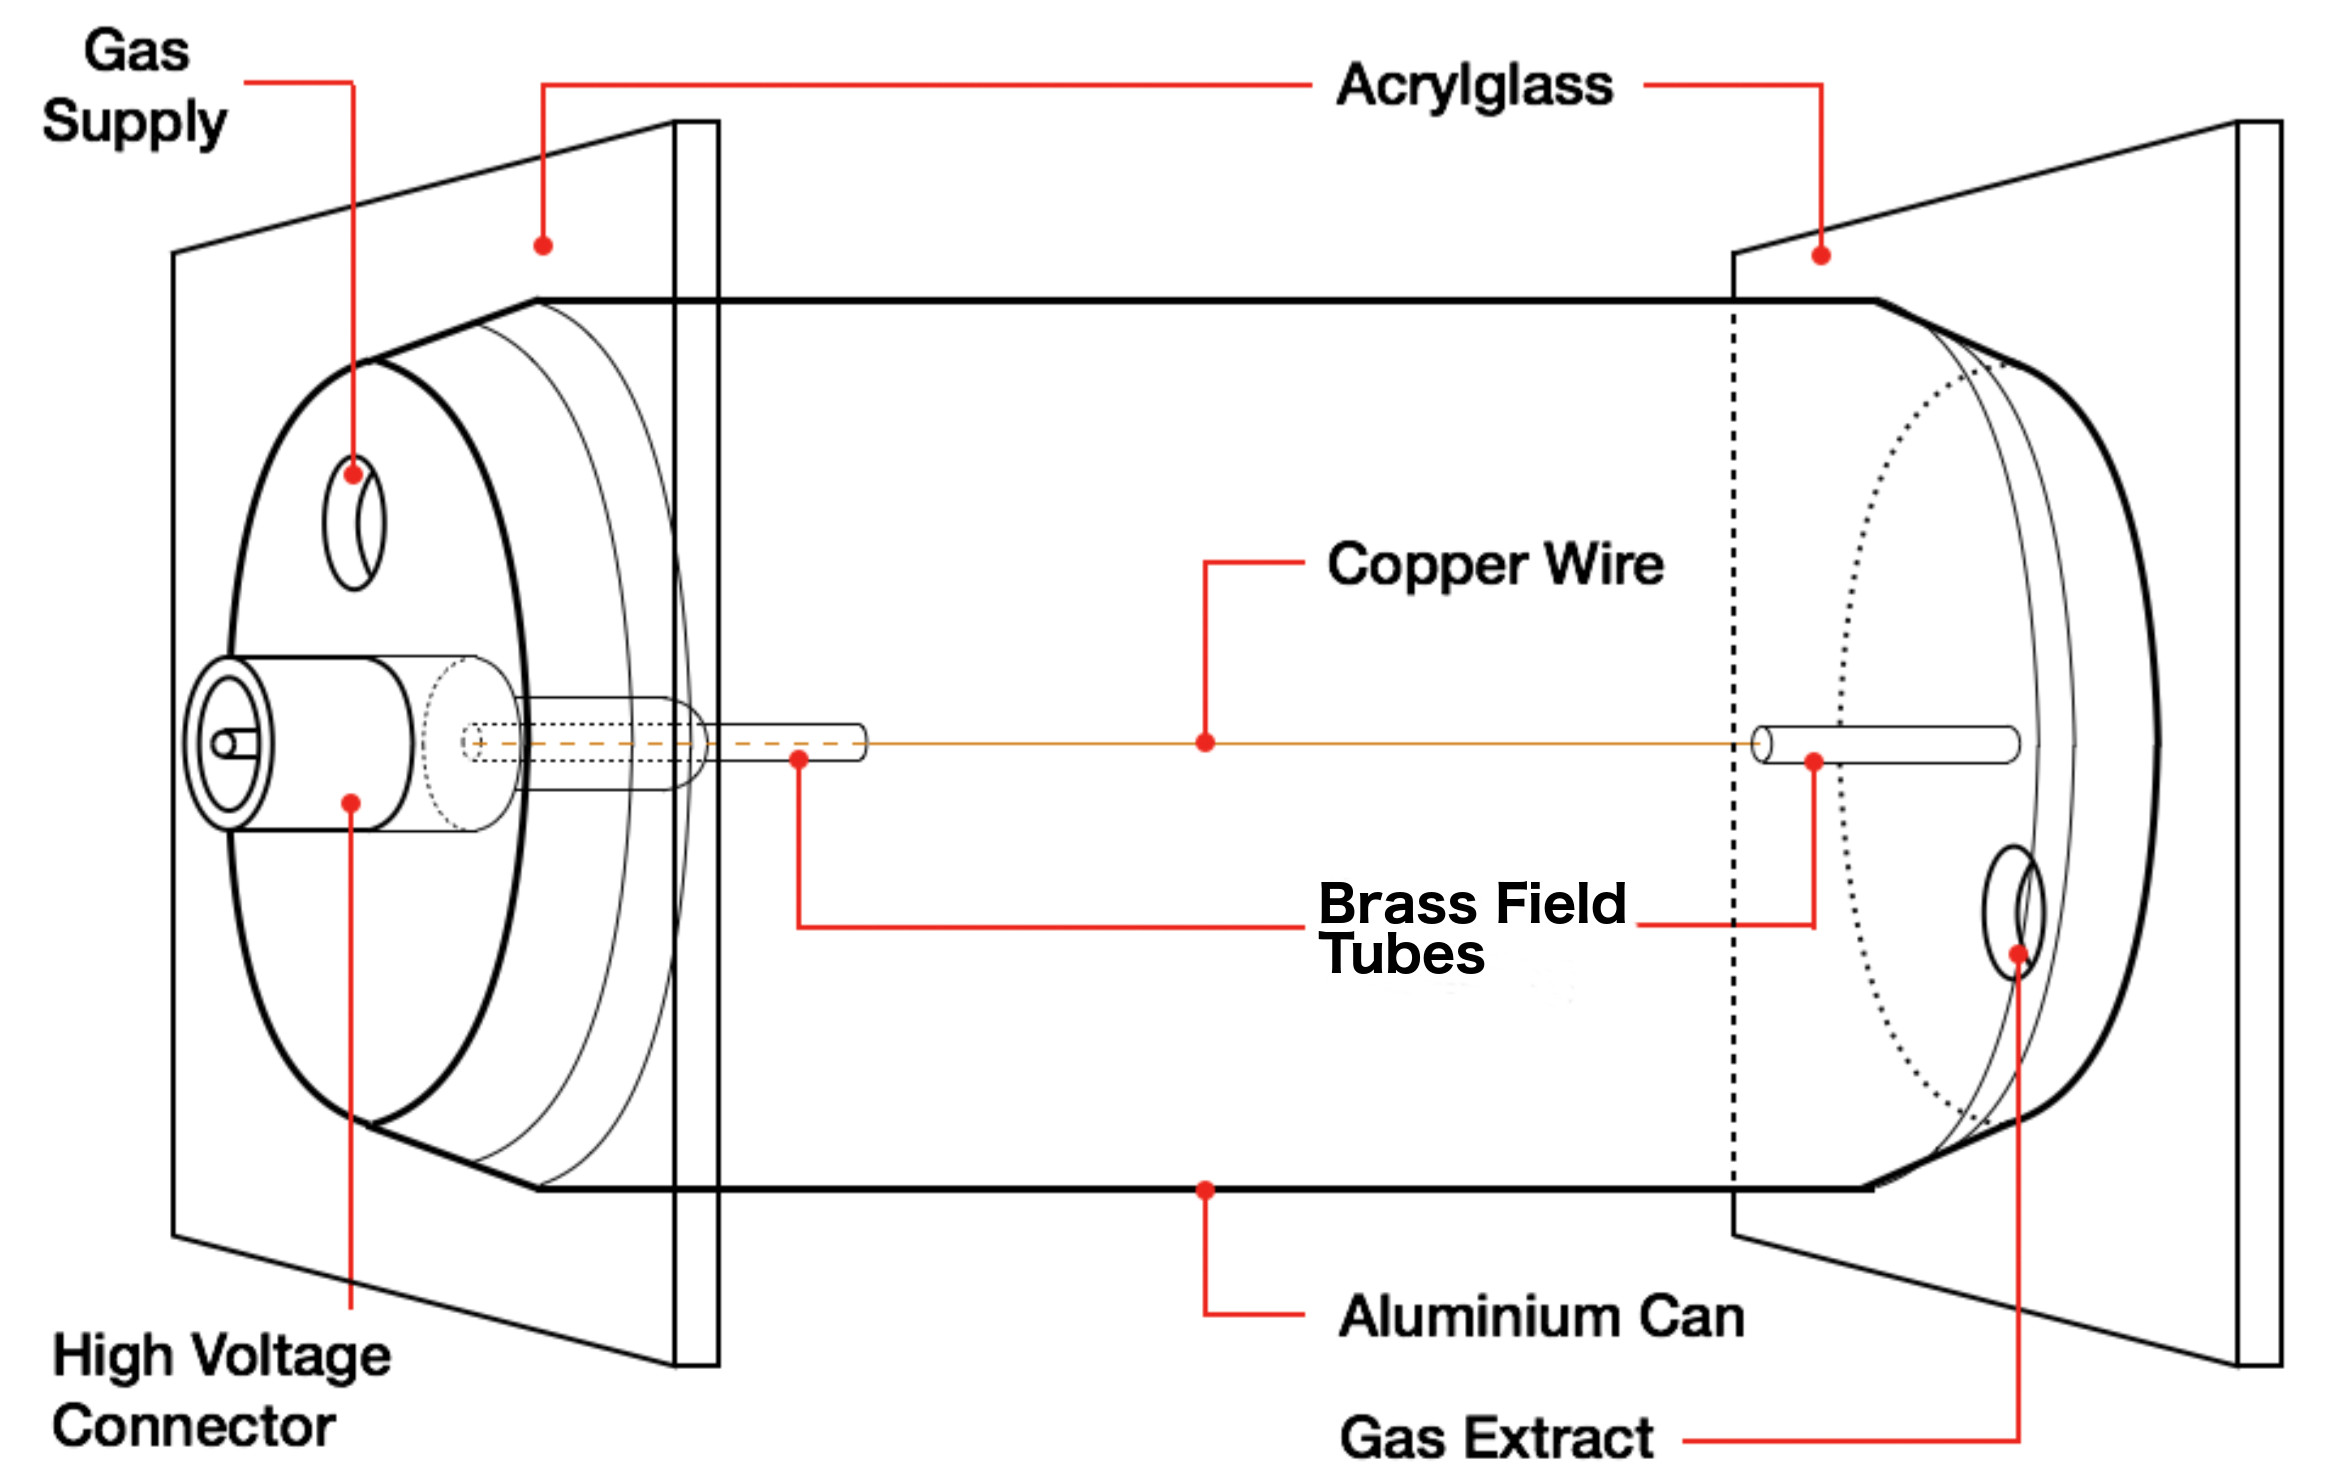
\includegraphics[width=\textwidth]{fig/instructions/schematic.png}
\caption{Schematic of the detector \cite{instructions}, TODO draw own one with vector graphics}
\label{fig:schematic}
\end{figure}

TODO: which form is the best: active or passive, and we or I? Is it a bad practice to use both active and passive?

First we prepared the parts of the detector by removing a single strand from a copper wire and cutting two pieces of brass tube for the wire mounting.
The course organizers removed the top of the can and drilled two holes to its bottom, one to the center and one off-center.
We then smoothened the cutting edges and grinded away the anti-corrosion layer from the inside of the walls of the can.
Table \ref{table:sizes} contains some size measurements of the can and the brass tubes.
The can thickness and brass tube diameter were measured using a
\href{https://en.wikipedia.org/wiki/Micrometer}{micrometer}, and the rest were measured with a
\href{https://en.wikipedia.org/wiki/Calipers}{caliper}.

\begin{table}[ht!]
\centering
\caption{Size measurements
- TODO: should the original data be included here?
It doesn't fit on the page, so should the margins be made smaller?
}
\begin{tabular}{l|l|l}
Measurement & $\mu$ & $\sigma$ \\
% \begin{tabularx}{\textwidth}{l|lllll|l|l}
% Measurement & \multicolumn{5}{l}{Data} & $\mu$ & $\sigma$ \\
\hline
Can outer diameter (mm)
% & 66.01 & 65.74 & 65.81 & 65.70 & 65.89
& 65.83 & 0.11 \\
Can top end inner diameter (mm)
% & 47.50 & 47.78 & 47.58 & 47.76 & 47.47
& 47.62 & 0.13 \\
Can top end outer diameter (mm)
% & 53.84 & 53.88 & 53.98 & 53.89 & 53.82
& 53.88 & 0.06 \\
Can bottom end inner diameter (mm)
% & 45.51 & 44.93 & 45.40 & 45.43 & 45.47
& 45.35 & 0.21 \\
Can thickness (\textmu m, from top section)
% & 240 & 250 & 240 & 250 & 280
& 252 & 15 \\
Can thickness (\textmu m, from cut can)
% & 102 & 103 & 102 & 100 & 102
& 101.8 & 1.0 \\
Long brass tube length (mm)
% & 29.25 & 29.26 & 29.27 & 29.27 & 29.25
& 29.26 & 0.09 \\
Short brass tube length (mm)
% & 10.05 & 9.98 & 9.99 & 9.99 & 10.04
& 10.02 & 0.03 \\
Brass tube diameter (µm)
% & 992 & 990 & 991 & 990 & 987
& 990.0 & 1.7 \\
Brass tube + connector length from acryl (mm)
% & 27.30 & 27.15 & 27.32 & 27.59 & 27.23
& 27.32 & 0.15 \\
% \end{tabularx}
\end{tabular}
\label{table:sizes}
\end{table}

Once the can and the other parts were ready, we put them to an ultrasonic cleaner for grease removal, as any leftover grease in the detector could interact due to the high-voltage conditions, causing degradation of detector performance.
To avoid contaminating the cleaned parts, every step from now on had to performed with rubber gloves.

We prepared the anode mounting by gluing the longer brass tube 
to the hole in the center of a plastic screw.
To avoid filling the hole within the brass tube, the outside of the brass tube was coated with glue, and the tube was then pushed into the hole.
The screw was then attached to the can with a plastic nut, as in figure \ref{fig:anode_mounting}.

\begin{figure}[ht!]
\centering
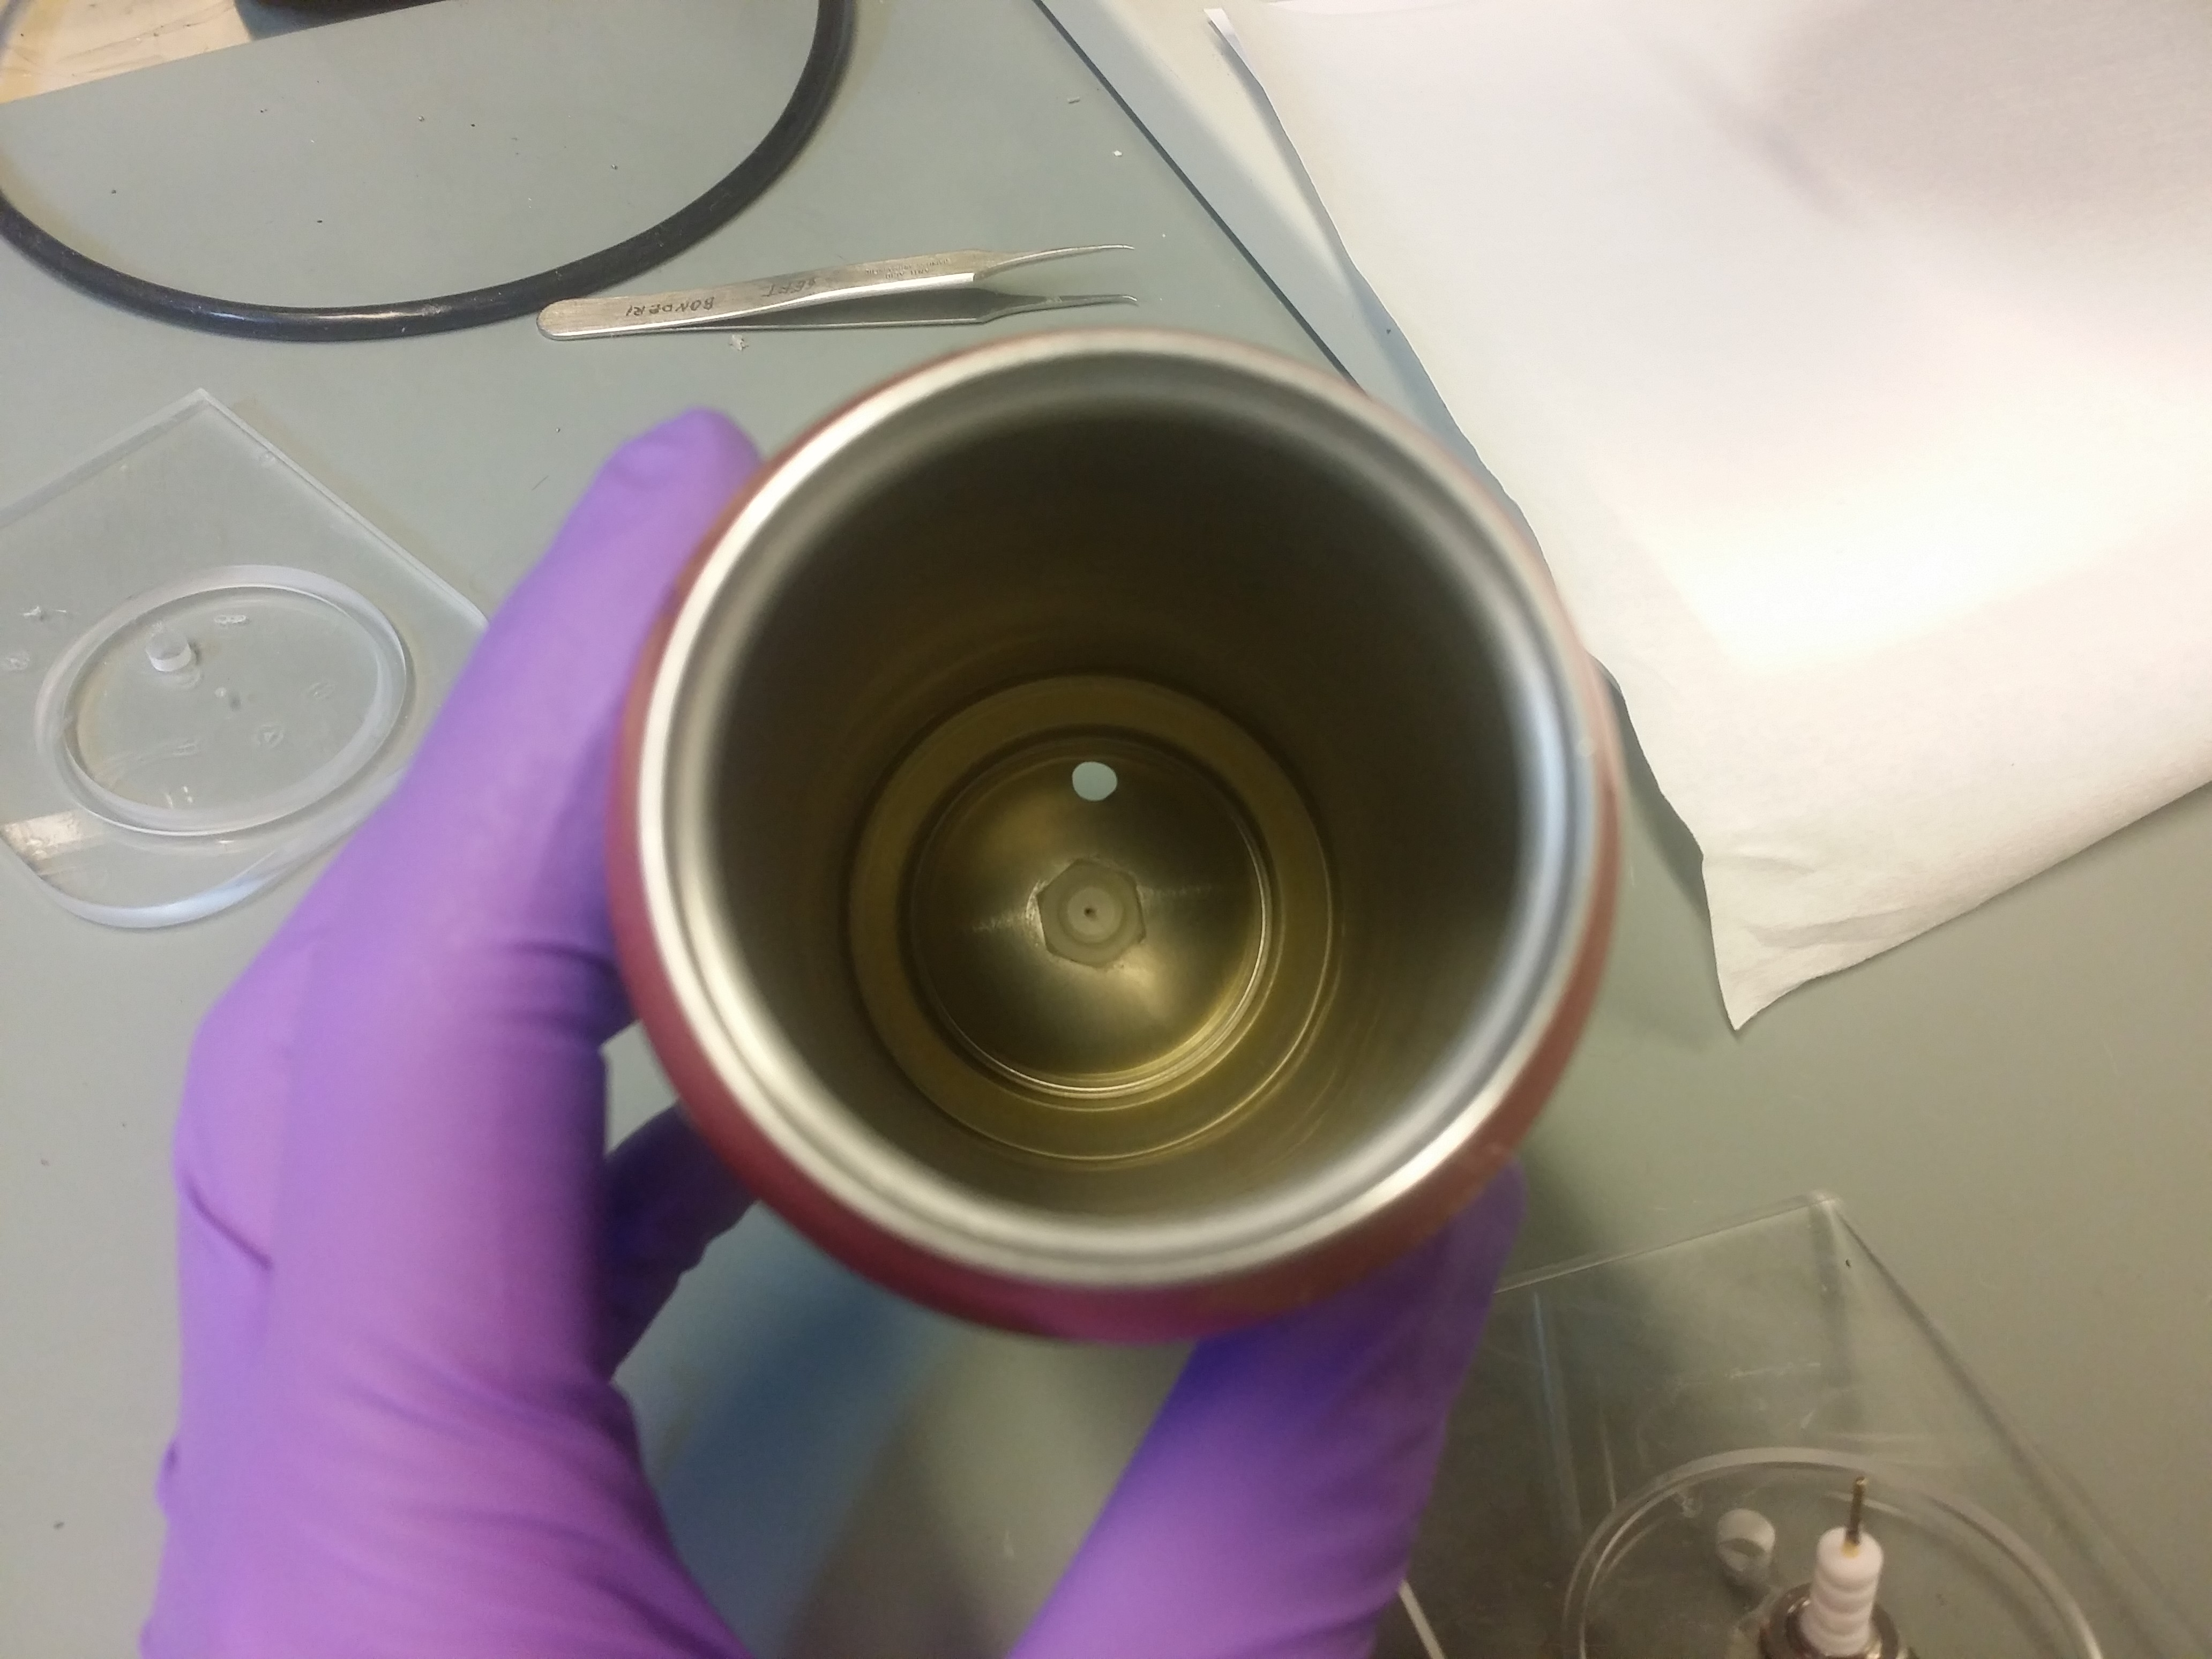
\includegraphics[width=\textwidth]{fig/IMG_20201123_103327.jpg}
\caption{A brass tube within a plastic screw serves as the other end of the anode wire}
\label{fig:anode_mounting}
\end{figure}

The electric connection of the anode would be supplied by a high-voltage coaxial connector, which we attached to one of the
\href{https://en.wikipedia.org/wiki/Poly(methyl_methacrylate)}{plexiglass}
end caps with a nut and some epoxy glue.
The nut is sufficient to keep the connector in place, but the glue makes the connection airtight.
Once the connector was in place, we pushed the anode wire through the brass tube at the bottom of the can and pulled it out of the top of the can.
We then pushed the wire through the shorter brass tube and twisted it into a hook so that it stayed in place when we pushed the brass tube into the connector.
The electrical connection was then formed by soldering the brass tube and therefore also the wire to the connector as in figure \ref{fig:connector}
In this step one should be careful not to leave the end of the wire exposed from the solder, as such a sharp tip would cause high electric fields and therefore undesired reactions within the detector.

\begin{figure}[ht!]
\centering
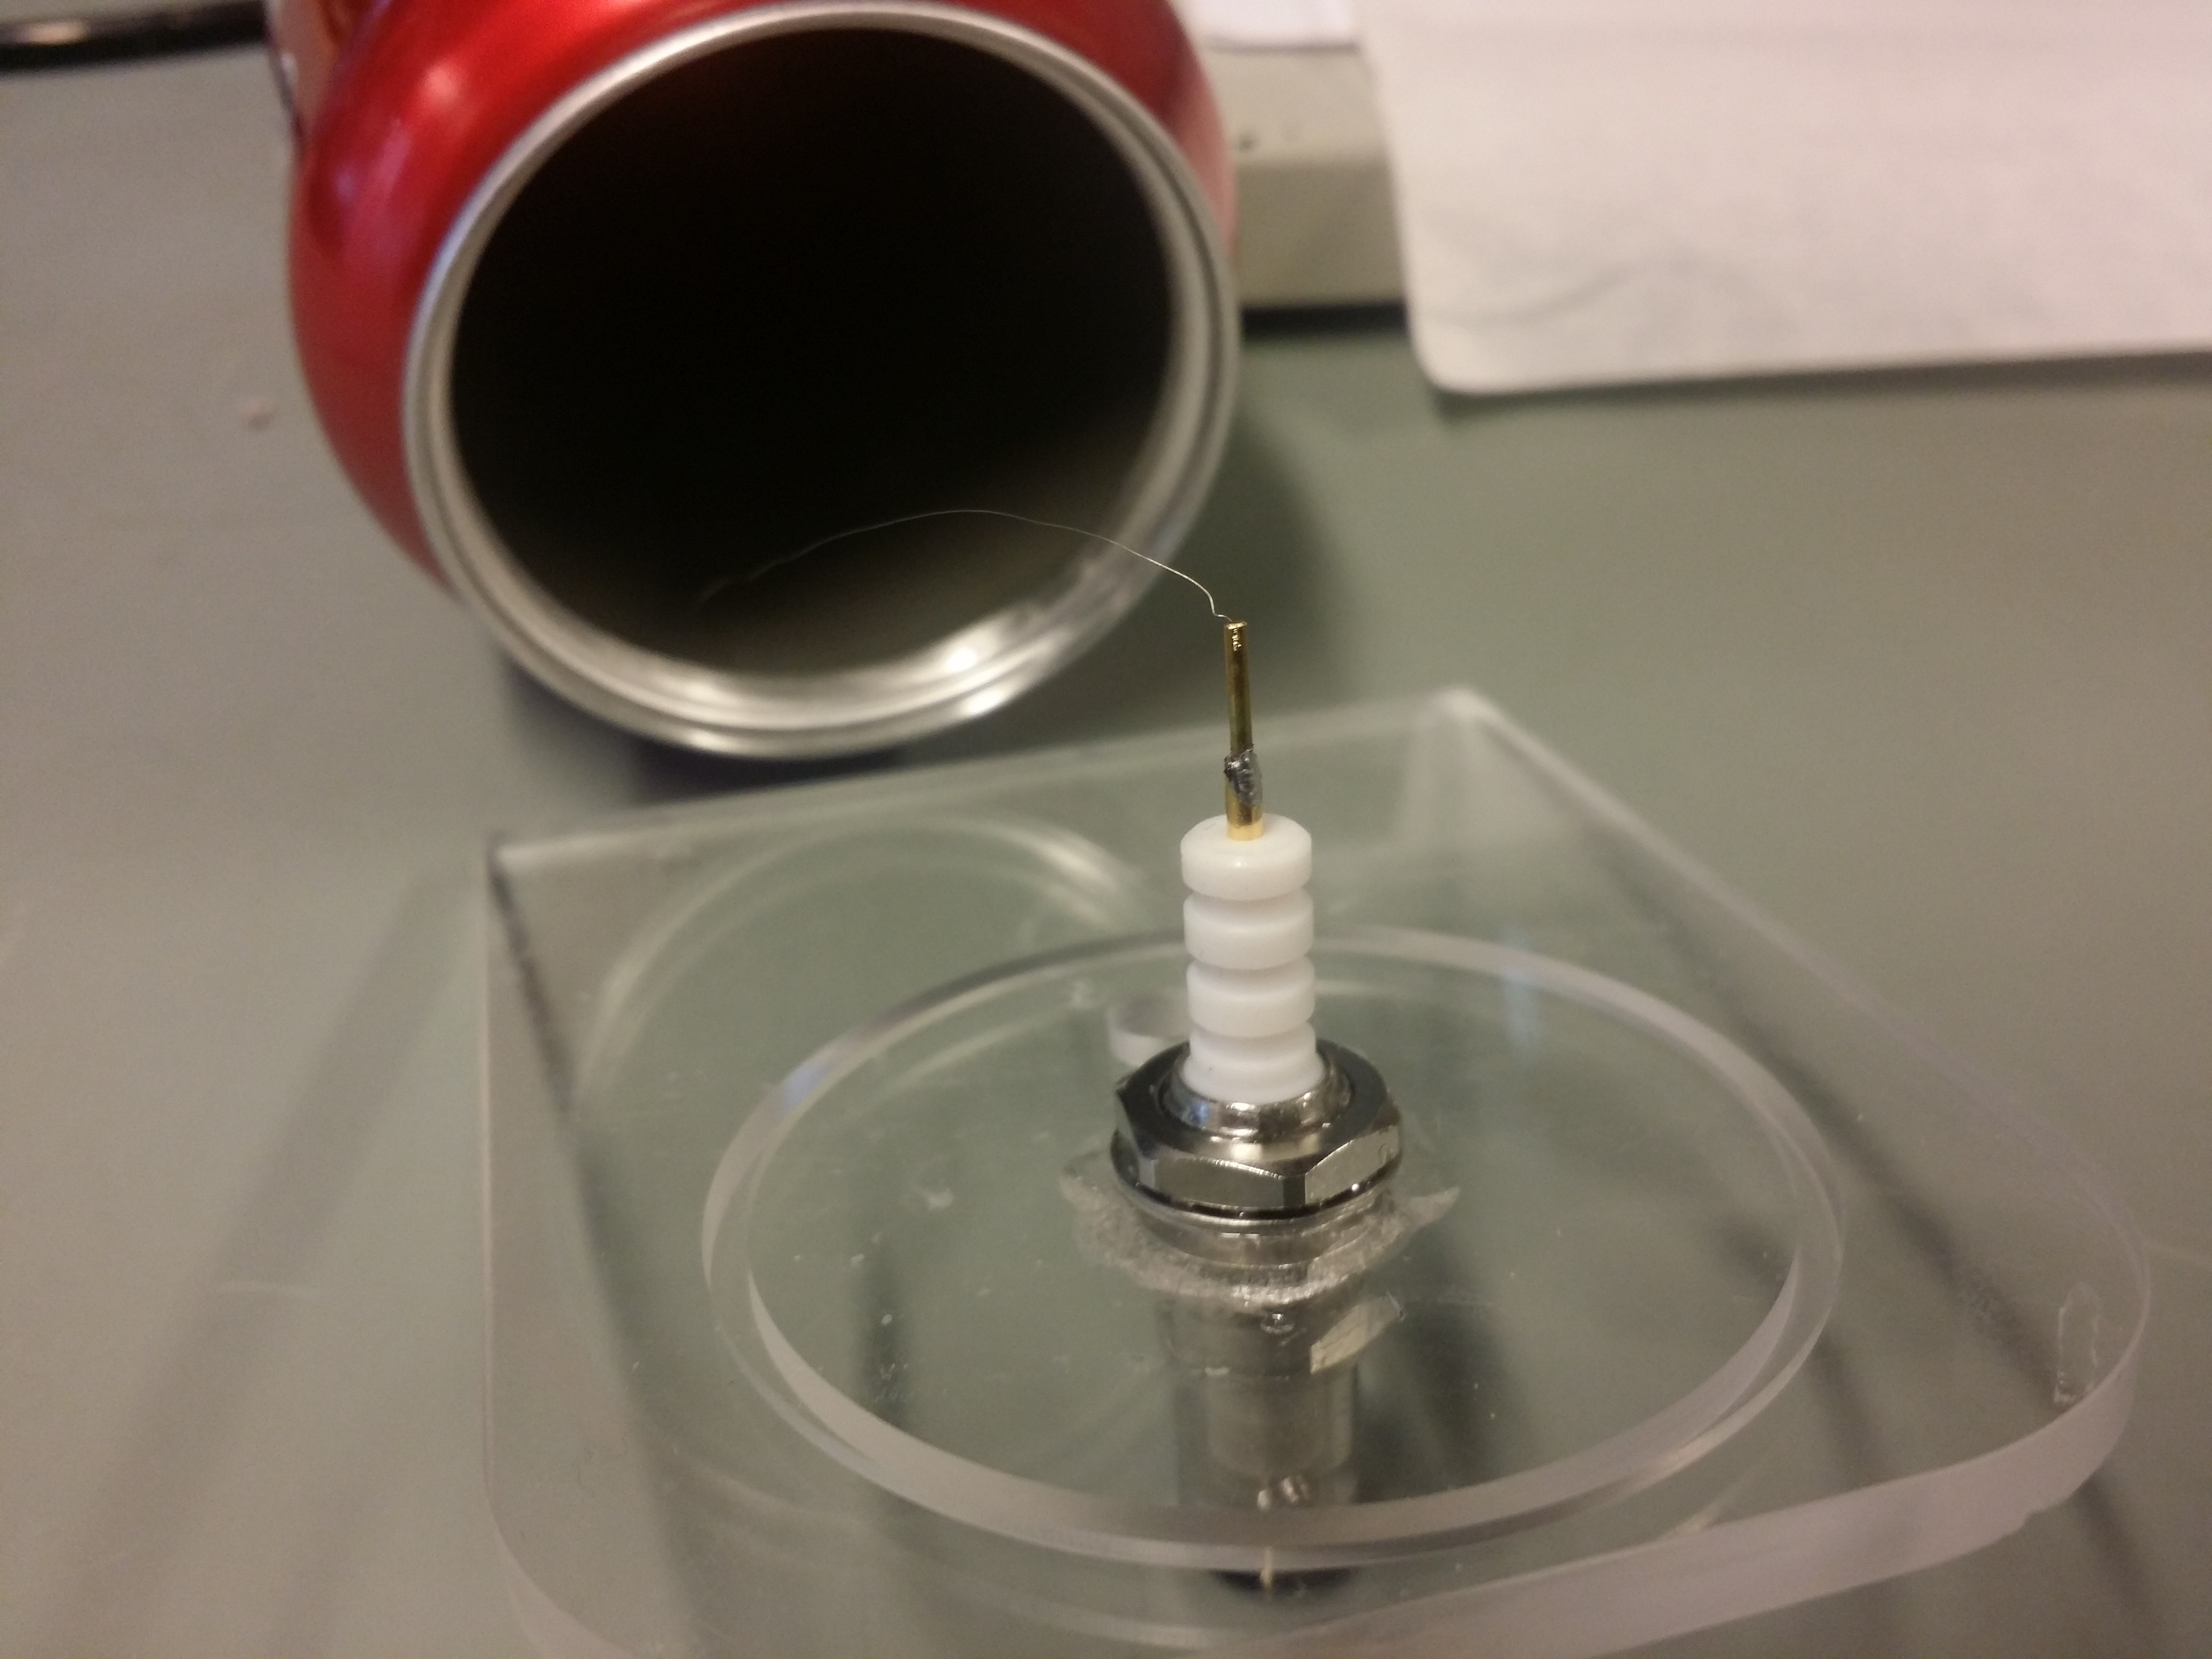
\includegraphics[width=\textwidth]{fig/IMG_20201117_121044.jpg}
\caption{The anode wire is soldered to the connector}
\label{fig:connector}
\end{figure}

Now the wire was in place, but it had to be tightened.
This was accomplished by taping the top cap to the can, knotting the wire around a nut and placing the wire over a wheel, as in figure \ref{fig:tightening}.
We then secured the tightening by soldering the wire to the brass tube, and then we cut the remaining wire.
In this step one should be careful to solder only as long as is needed for the solder to melt, as heating the wire for too long will cause it to break, as happened once during the manufacturing of this detector.
In the case of such an accident, a new wire has to be soldered to the high voltage connector.

\begin{figure}[ht!]
\centering
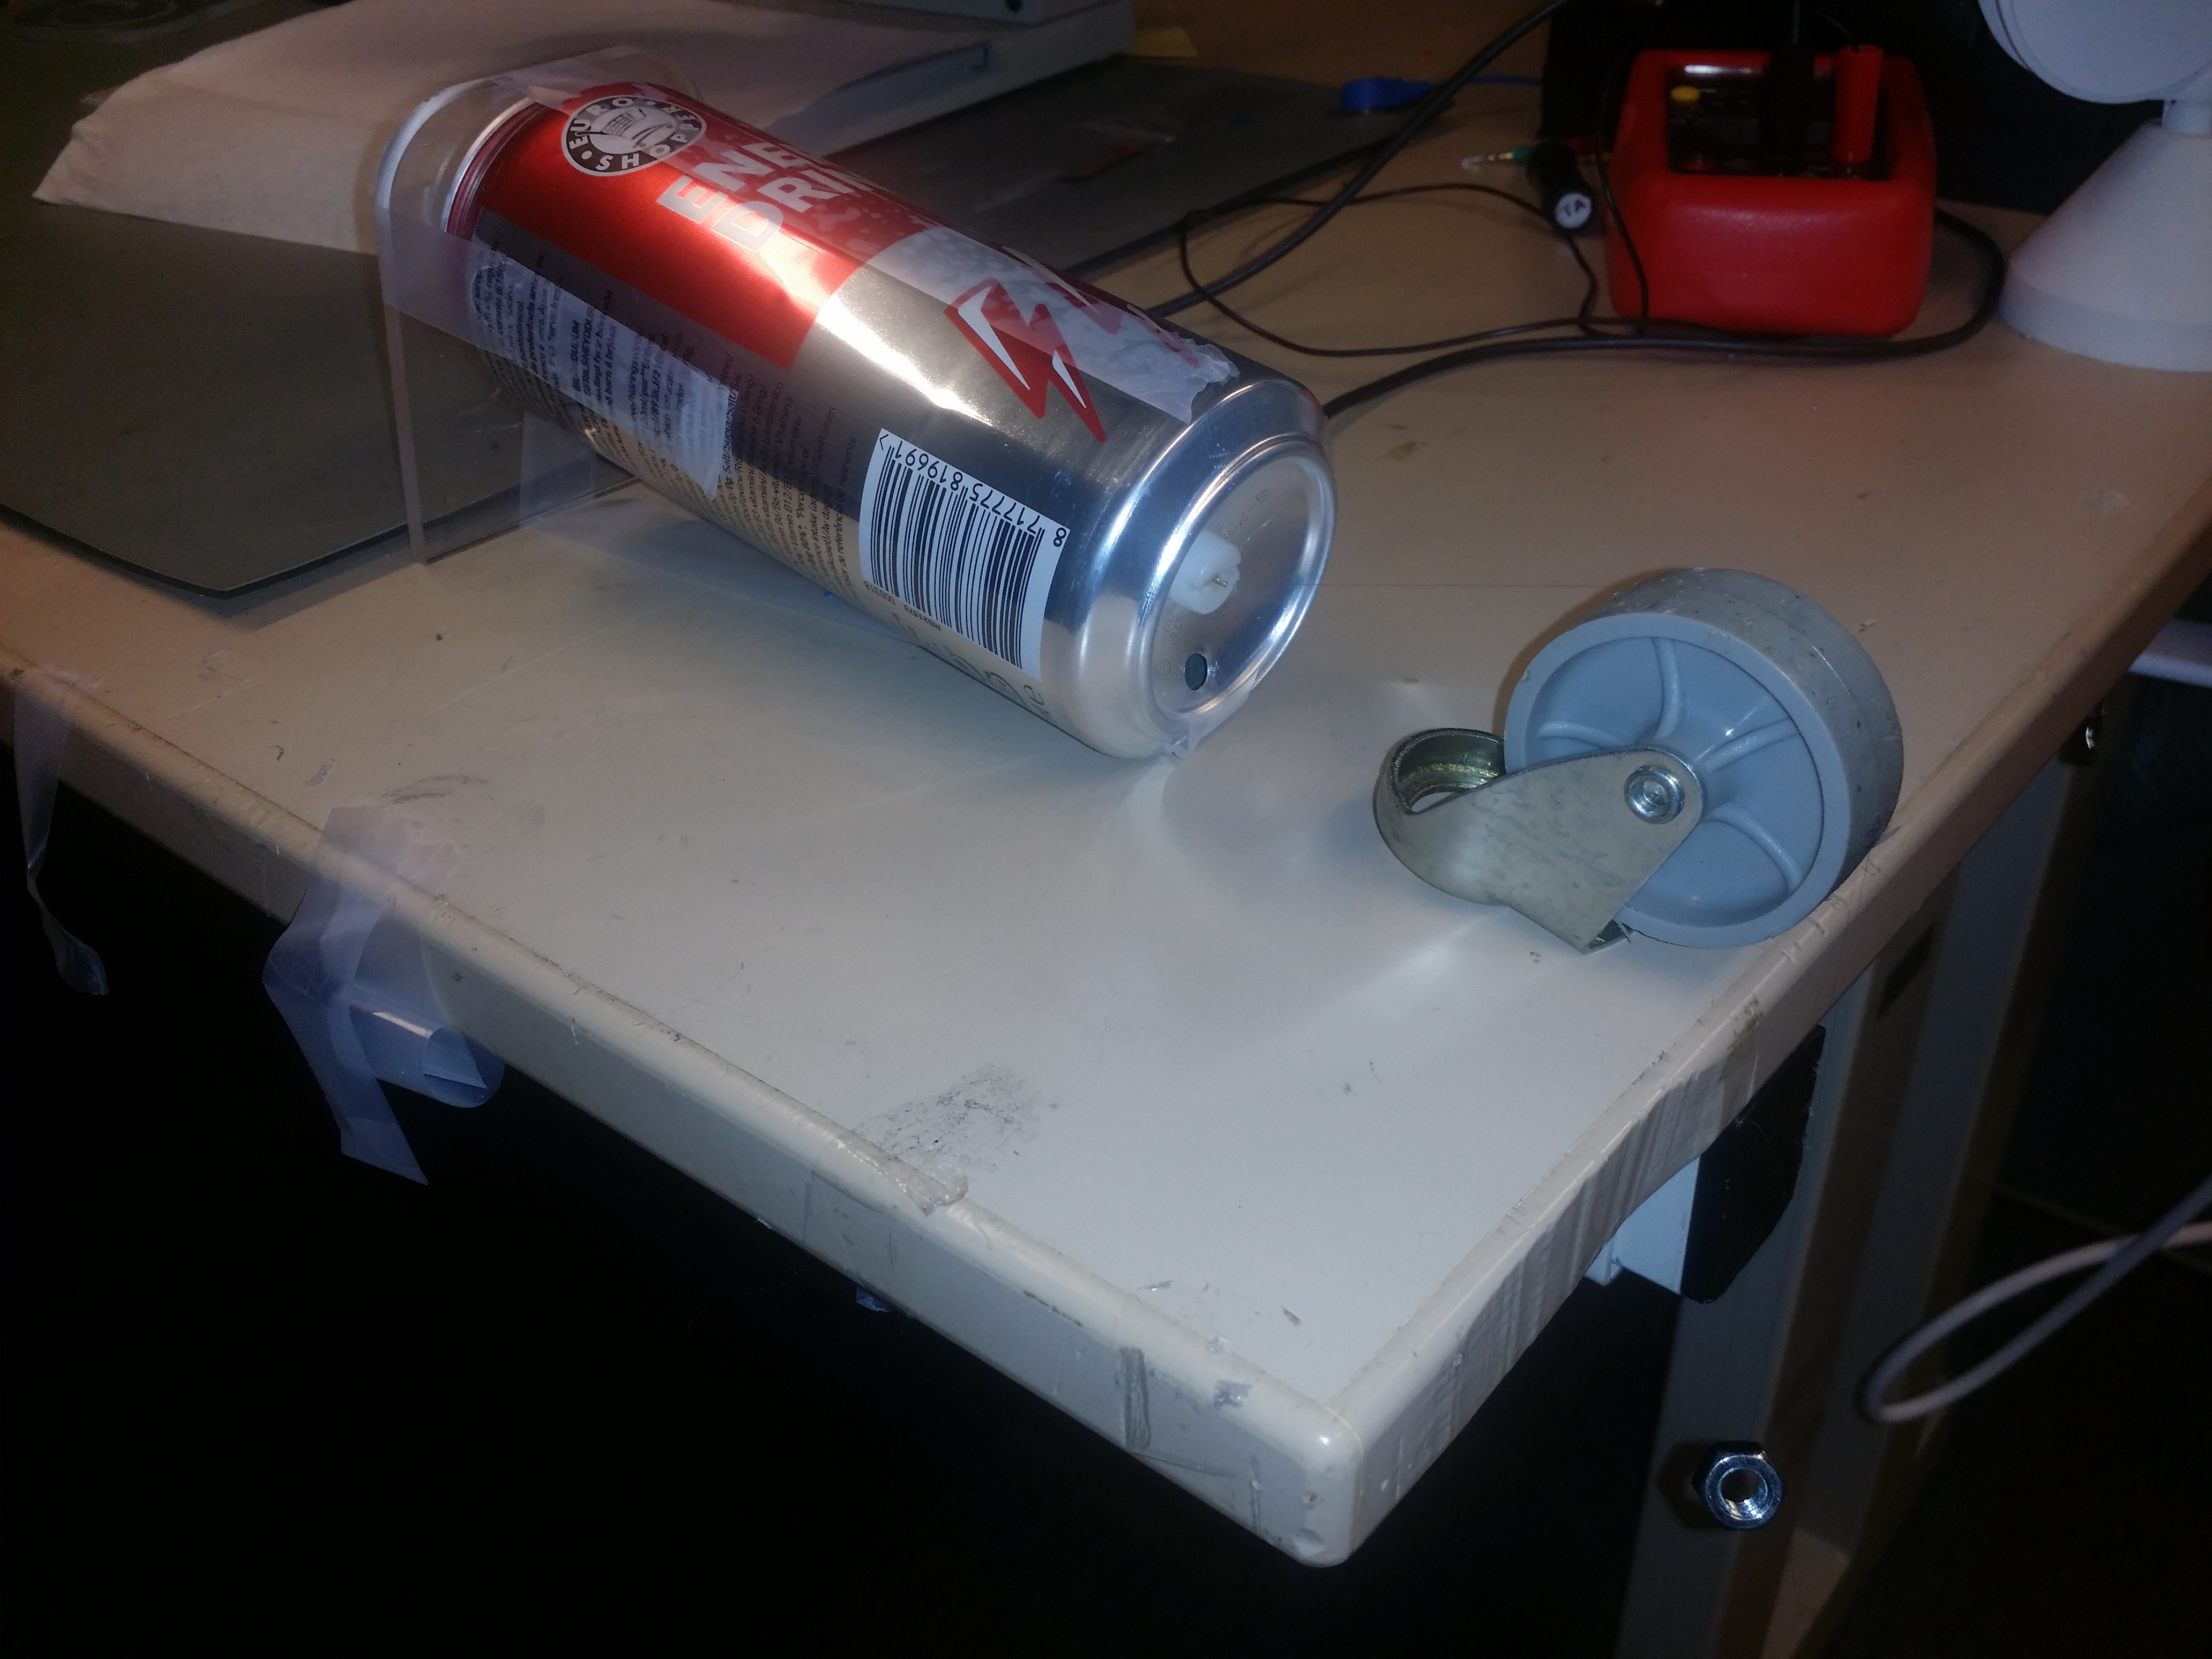
\includegraphics[width=\textwidth]{fig/IMG_20201123_104201.jpg}
\caption{Setup for tightening the anode wire}
\label{fig:tightening}
\end{figure}

Now the wire was in place, and the detector had to be sealed.
We used large amounts of epoxy to attach the end caps, and office tape to hold the caps in place.
In this step one should wait for the epoxy to dry properly before removing the top cap, as otherwise the cap may move and break the strained anode wire.
Once the epoxy of the caps was dry, we added some more to ensure airtightness, and then attached a pipe to the hole on each of the end caps.

Finally we brushed one side of the can with sandpaper and attached a piece of copper tape so that it went all the way to the shielding of the high voltage connector.
This established an electrical connection between the ground and the can.
It should be noted that the copper tape should be put on a different side as on which the radiation source is placed, as the copper tape would otherwise absorb some of the radiation.
A piece of aluminum foil was put over the bottom of the can to provide additional shielding from electromagnetic interference, as the end of the anode wire slightly extrudes from within the can.


\FloatBarrier
\subsection{Calibration}
The electronics have to be calibrated with an external pulser

\begin{figure}[ht!]
\centering
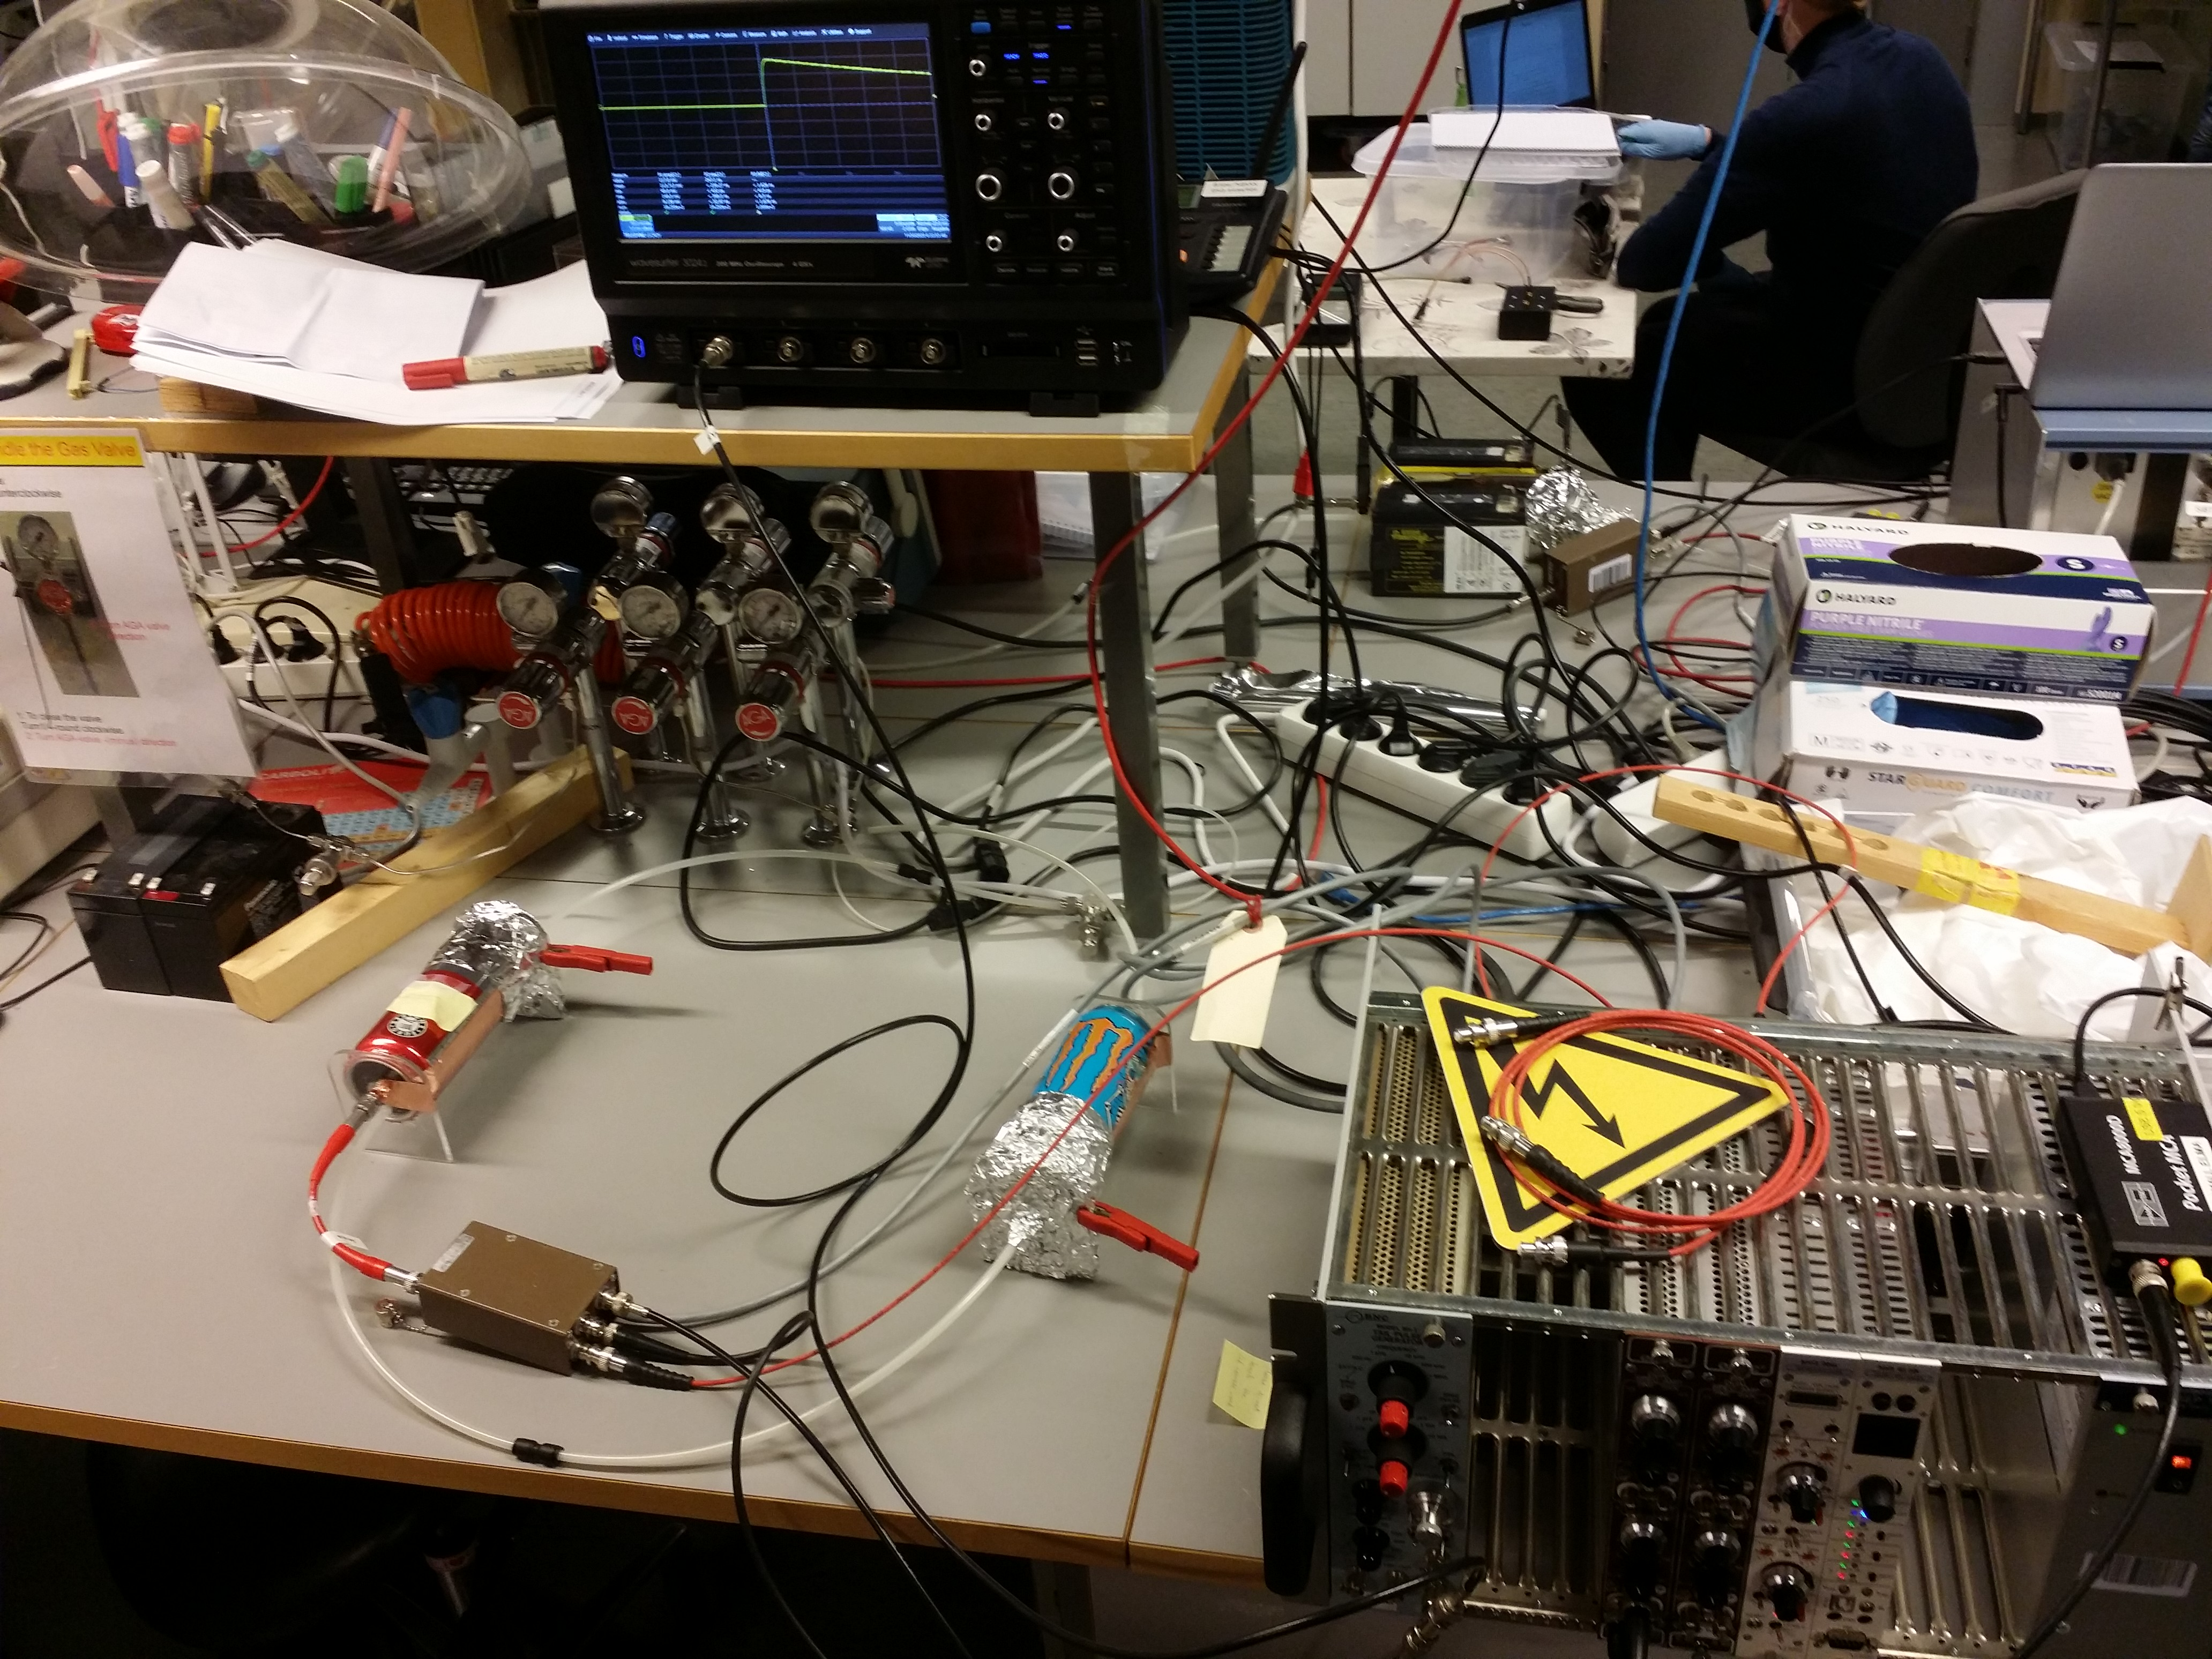
\includegraphics[width=\textwidth]{fig/IMG_20201130_135000.jpg}
\caption{Setup for testing with an external pulser}
\end{figure}


\FloatBarrier
\subsection{Testing}

\begin{figure}[ht!]
\centering
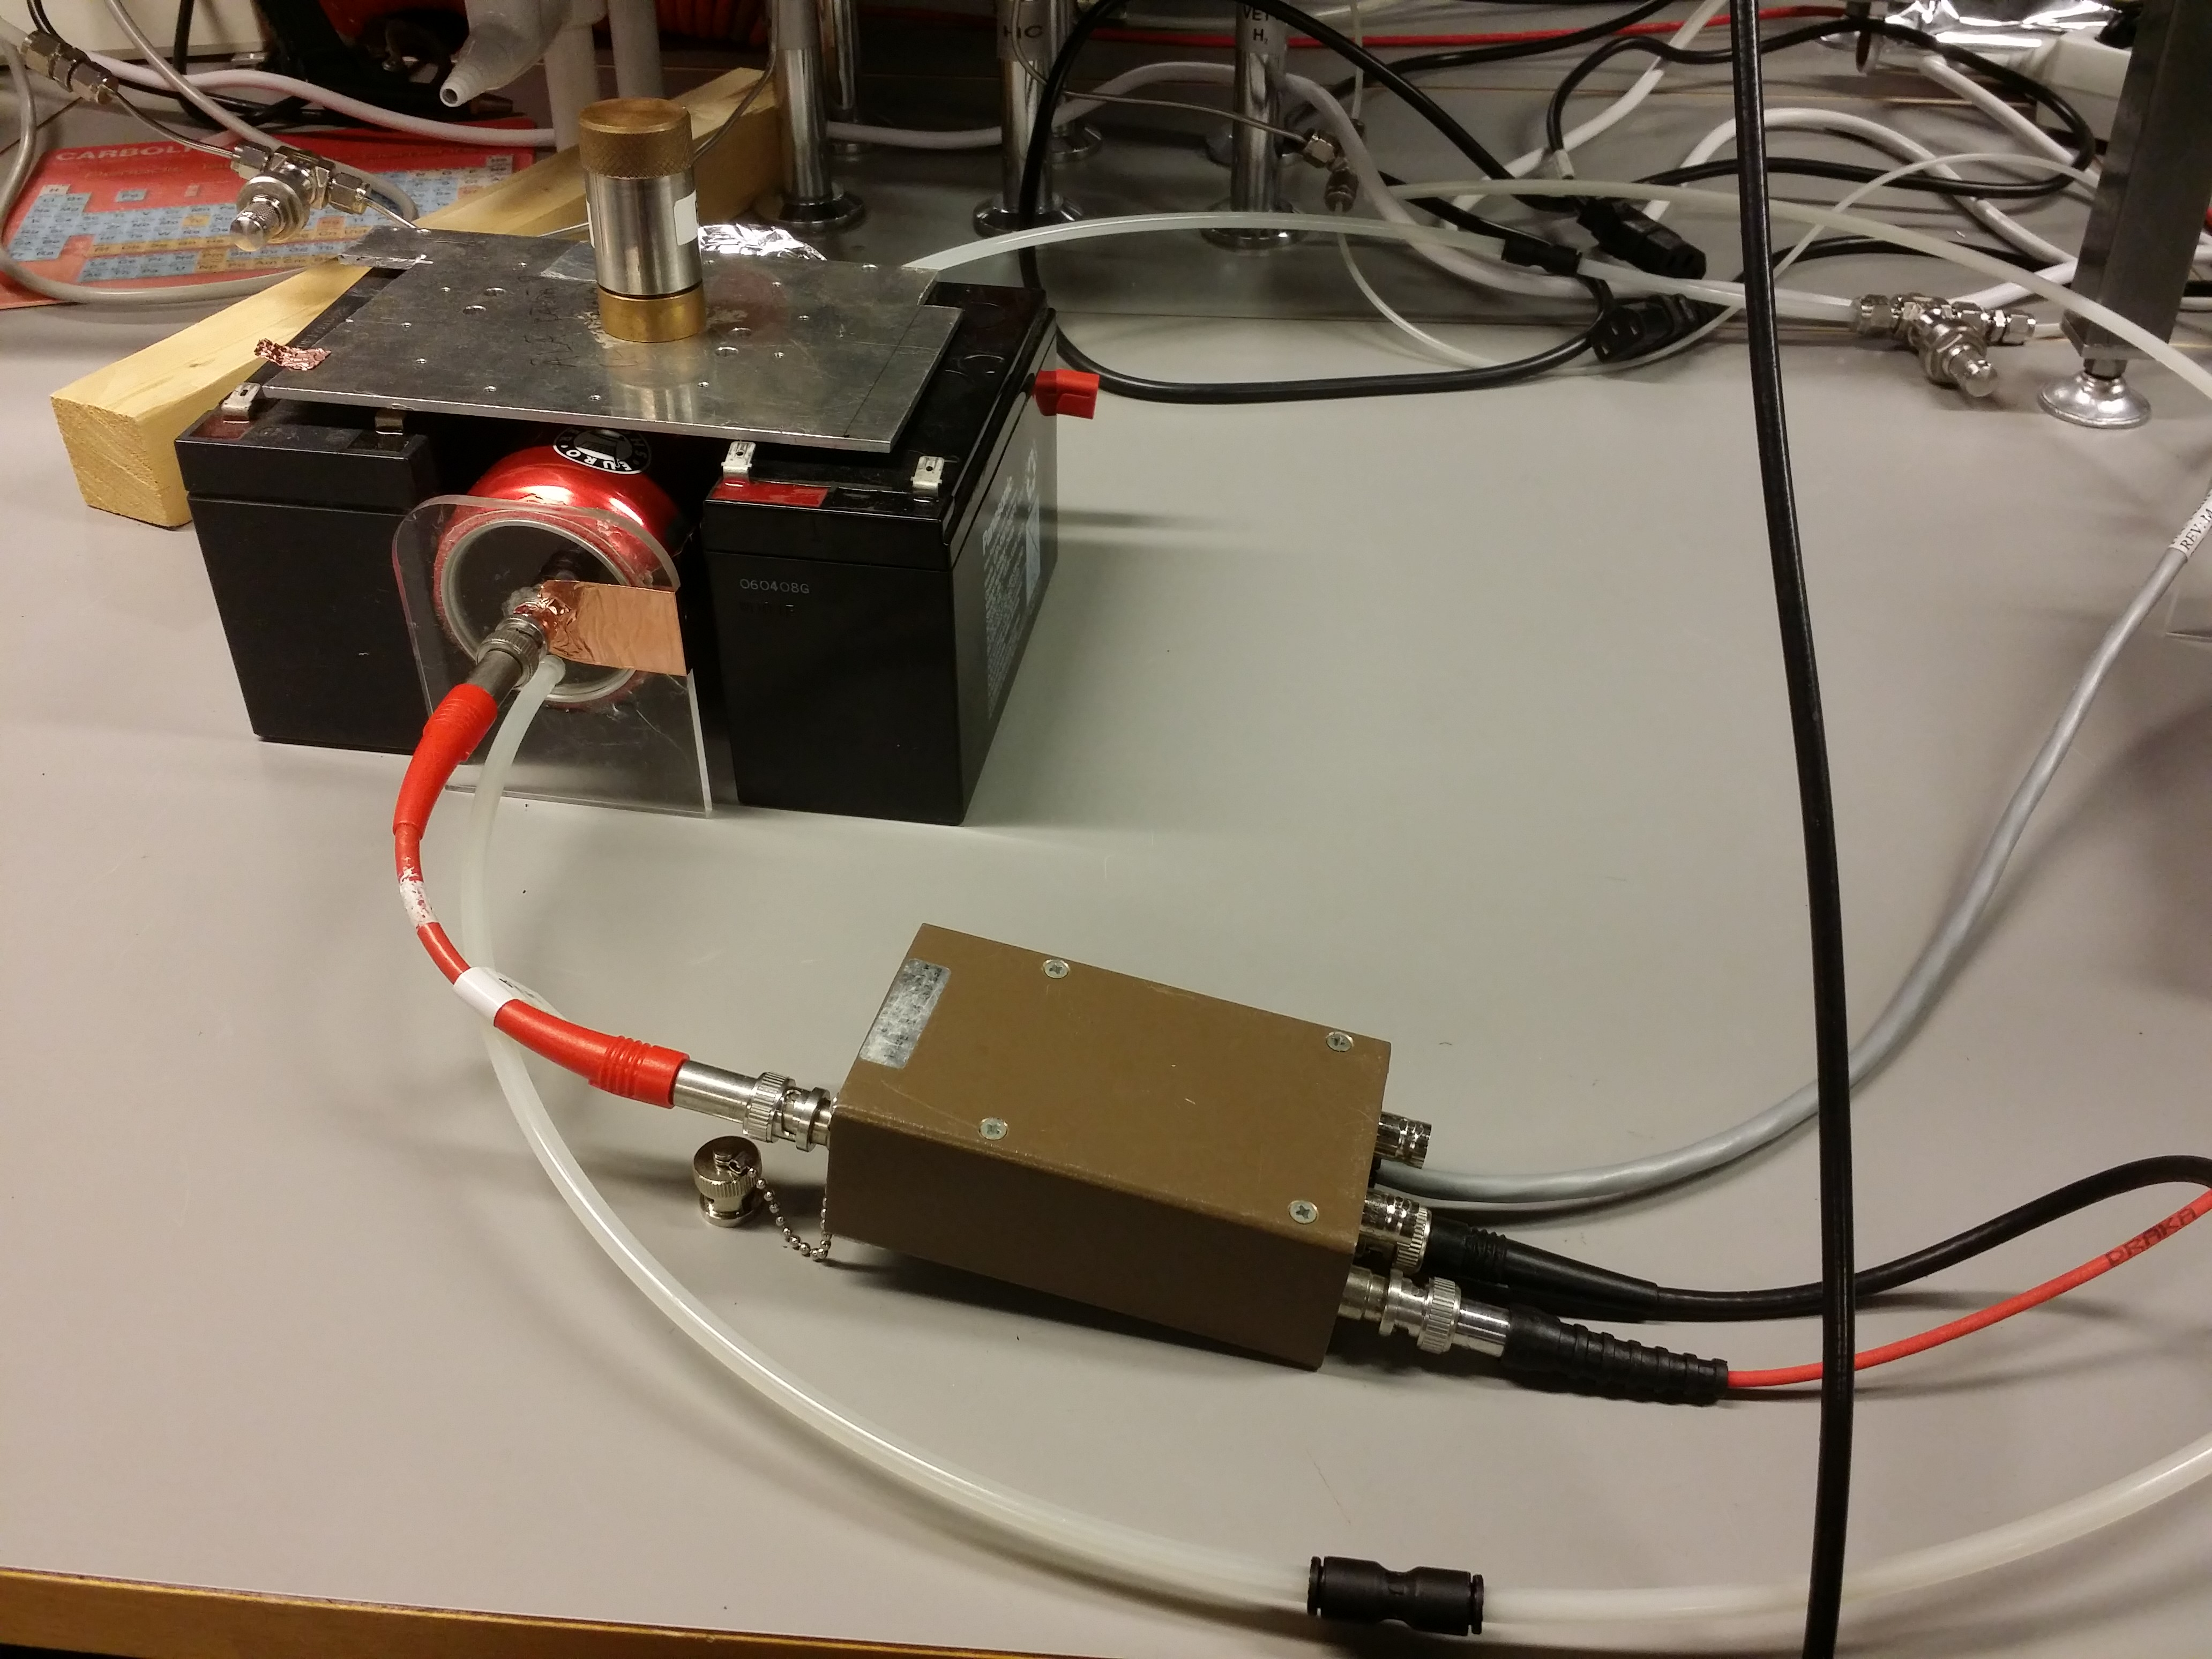
\includegraphics[width=\textwidth]{fig/IMG_20201130_144418.jpg}
\caption{Setup for testing with an Fe-55 source and a rack-mounted amplifier}
\end{figure}


\FloatBarrier
\section{Results and discussion}


\subsection{Calibration}
Output vs. input signal
See the spreadsheet!

\subsection{High voltage sweep}
The effect of gain settings and detector voltages

\subsection{Spectral measurement}
Some nice MCA spectra here
The uncertainty is not merely the width of the peak. We have to estimate all the uncertainties involved and propagate the errors.


\section{Conclusions}
Discuss results in context.
No need to repeat the results.
Refer to the introduction.
Was the aim fulfilled?
Were the results as expected? If not, why?
Is the mesurement precise enough to discuss ASDF?


\clearpage
\begin{appendices}

\section{Pre-amplifier}
\label{pre_amp}

Construction and detailed characterization here

\begin{figure}[ht!]
\centering
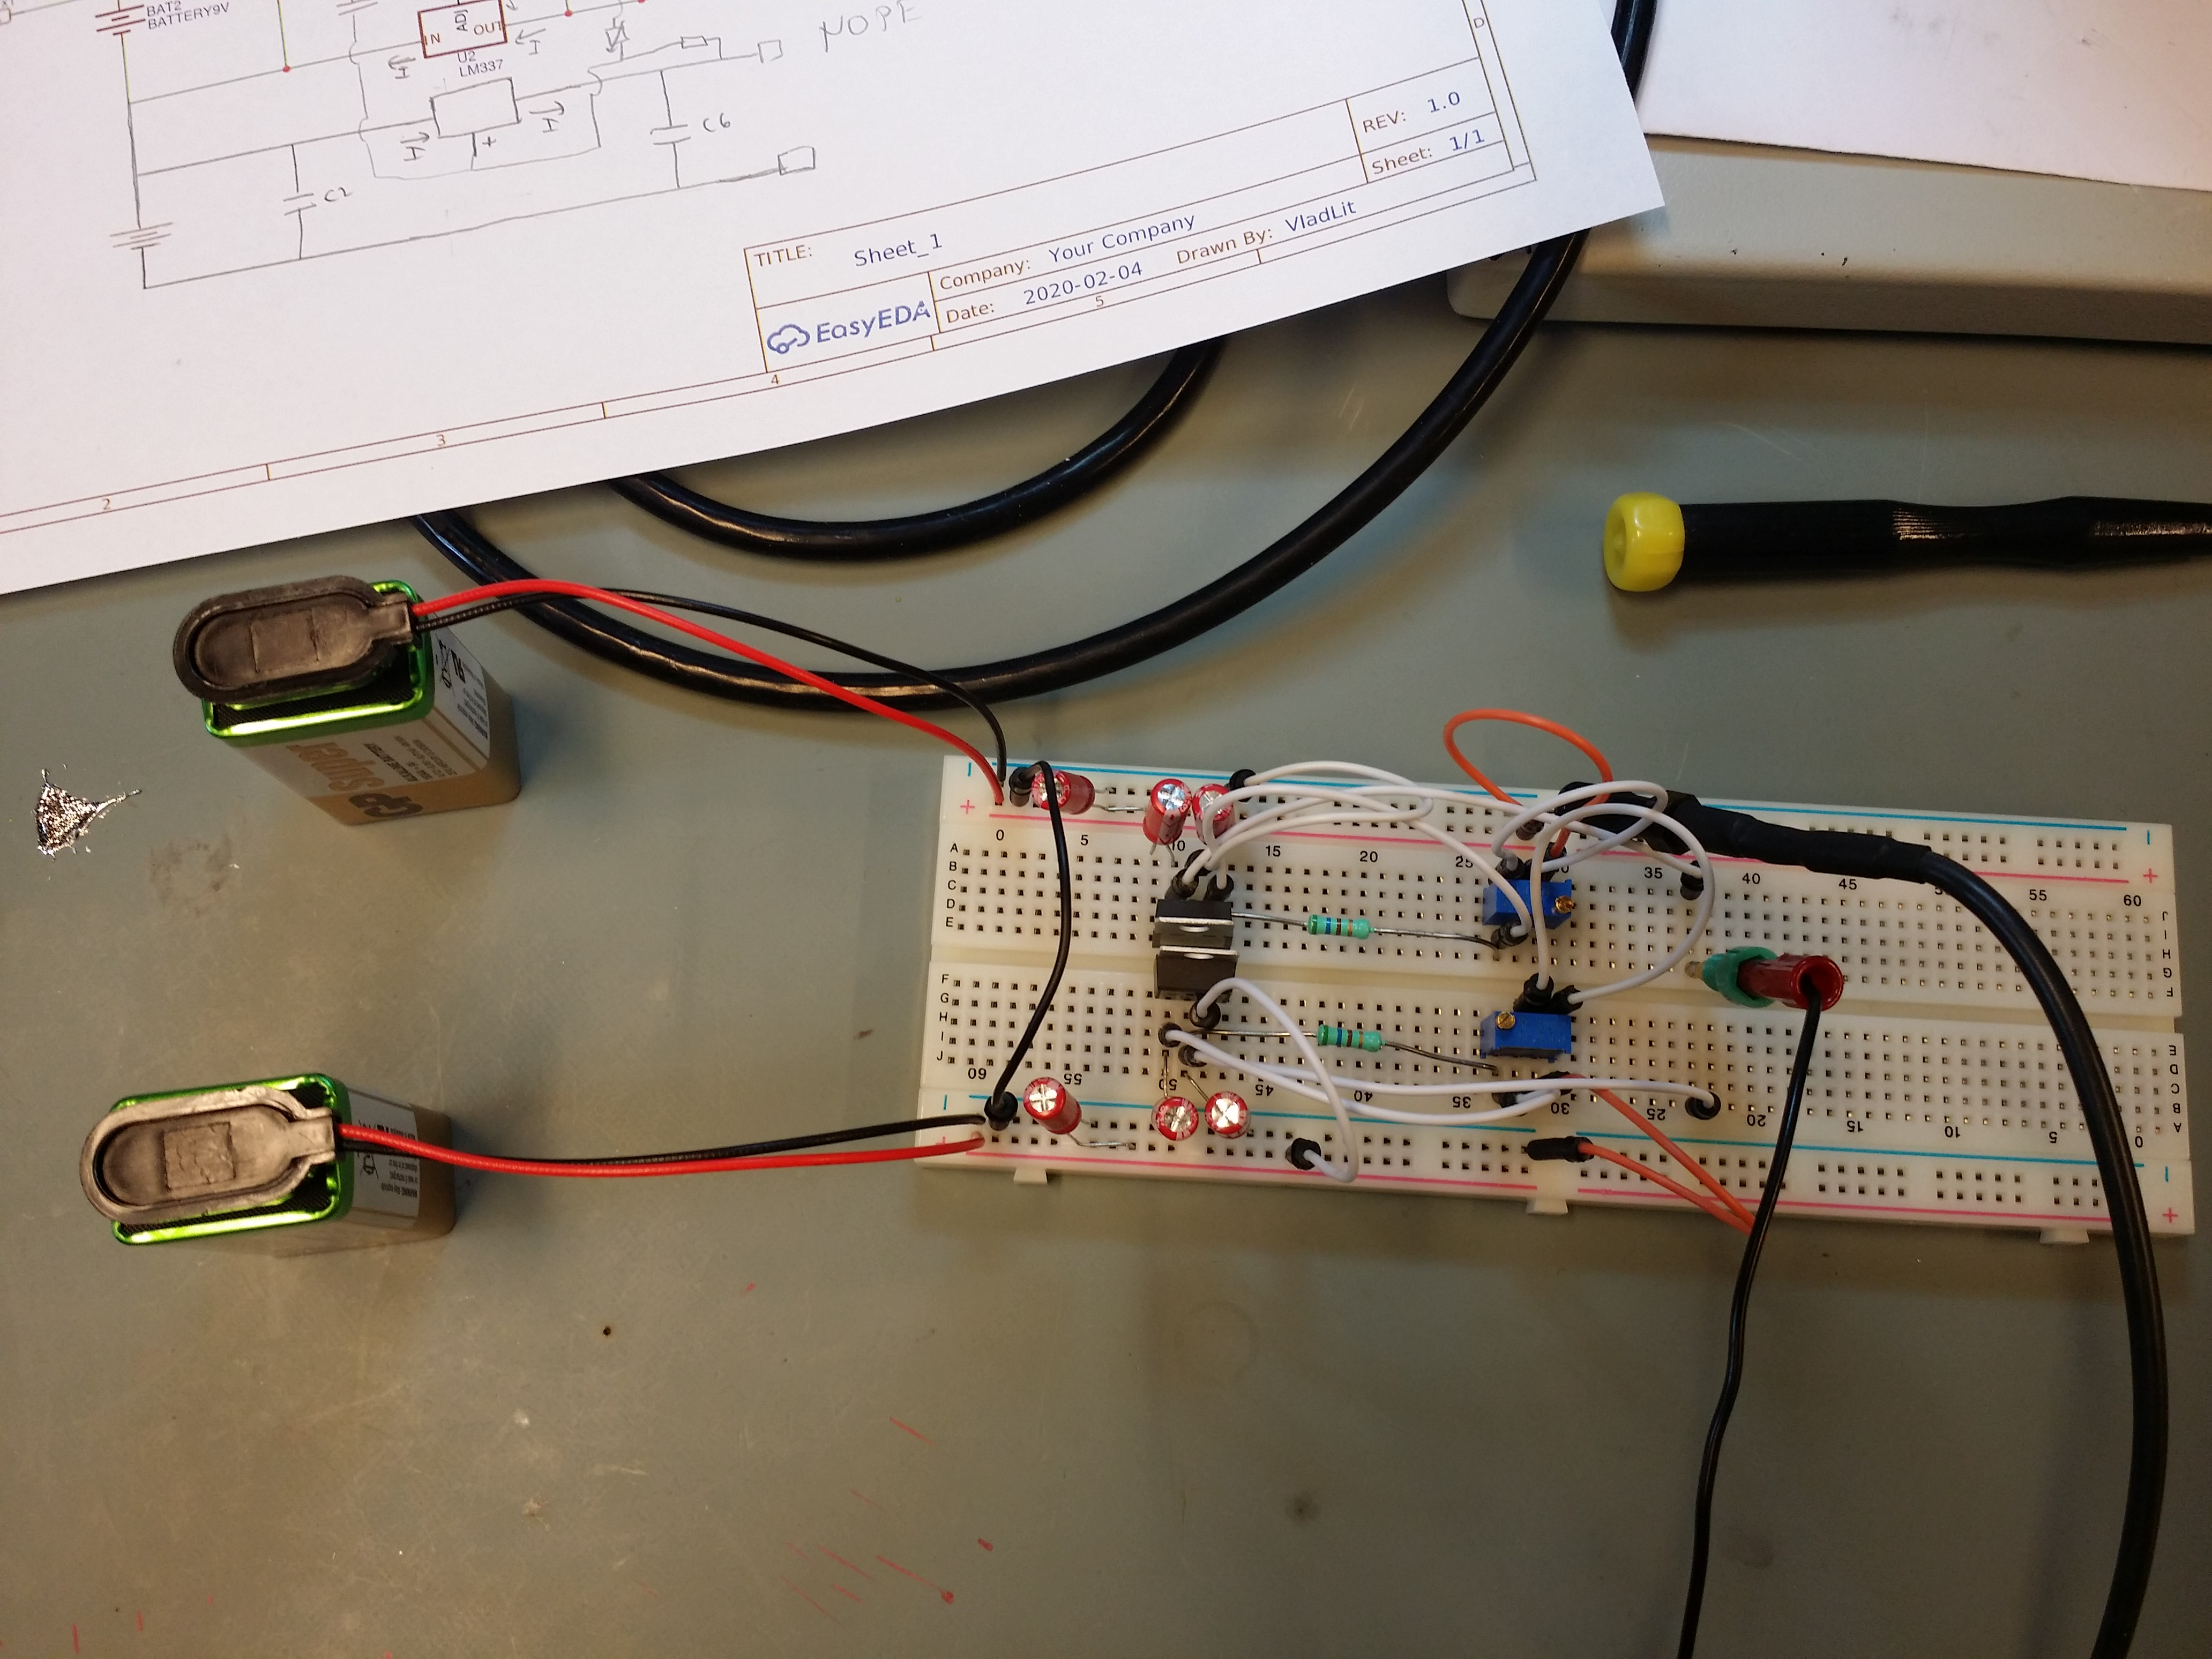
\includegraphics[width=\textwidth]{fig/IMG_20201005_104331.jpg}
\caption{Preliminary testing of the pre-amplifier components}
\end{figure}


\begin{figure}[ht!]
\centering
\subcaptionbox{}{
	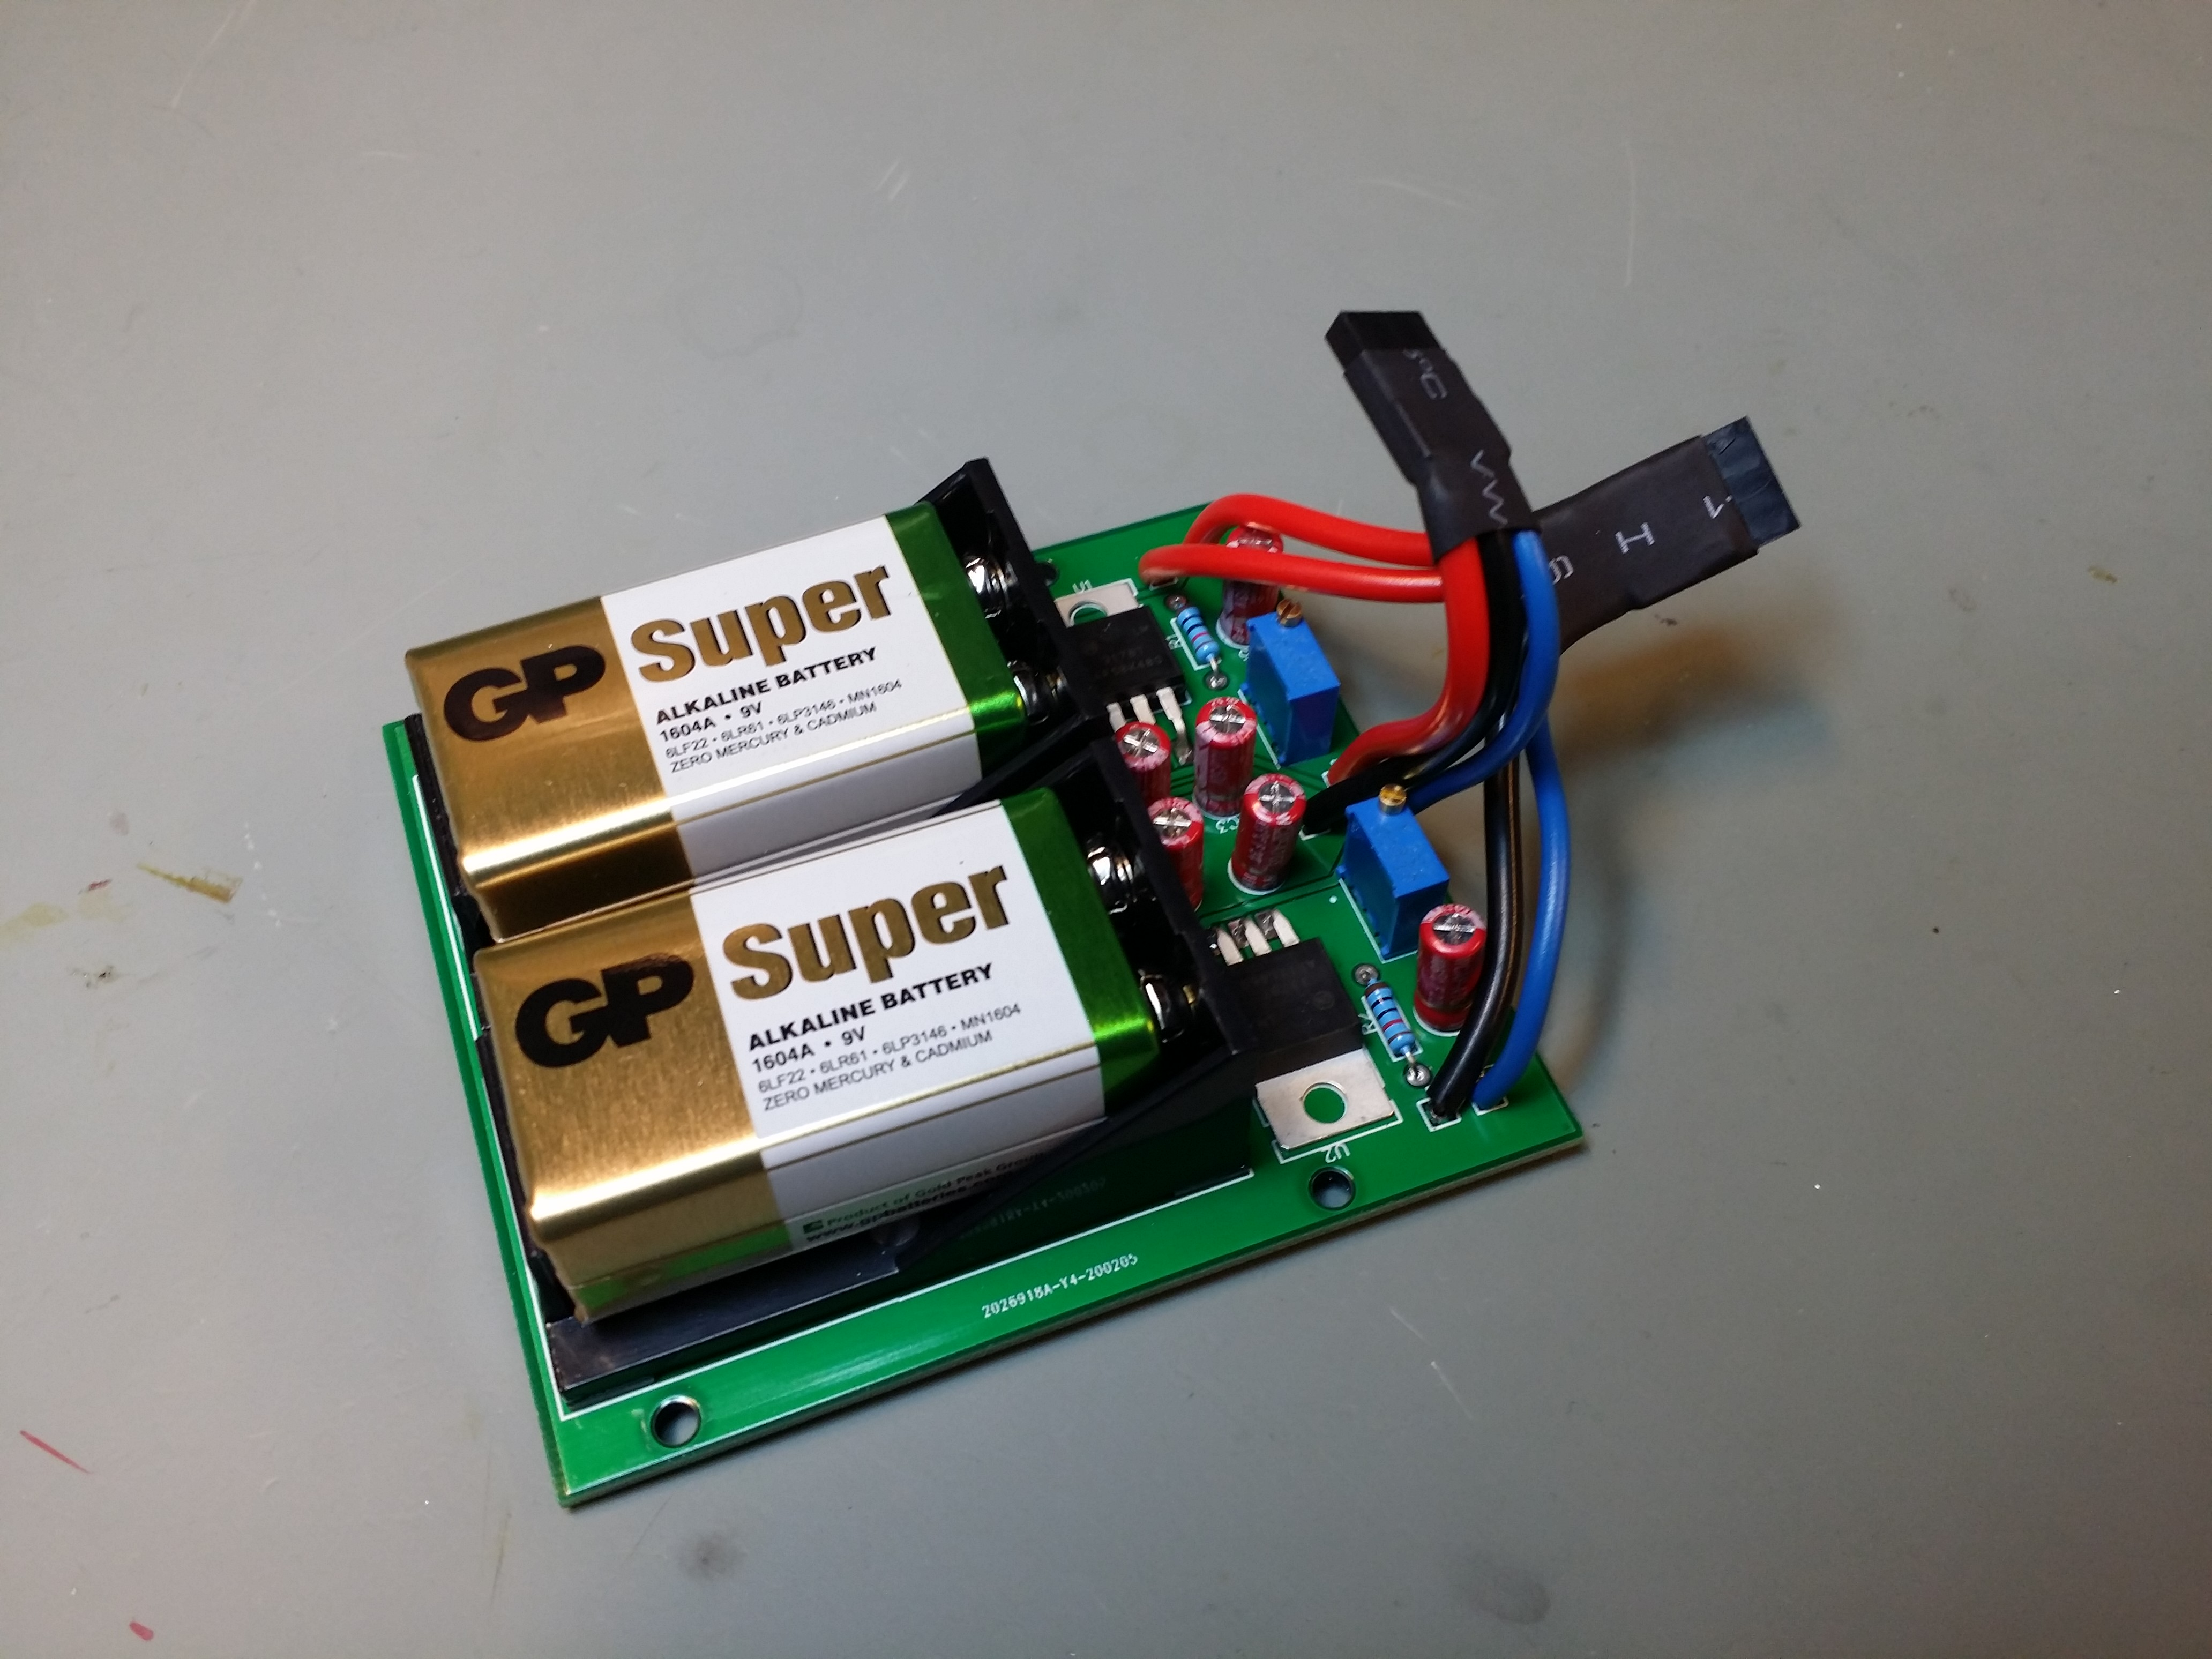
\includegraphics[width=\textwidth]{fig/IMG_20201201_121635.jpg}
}
\subcaptionbox{}{
	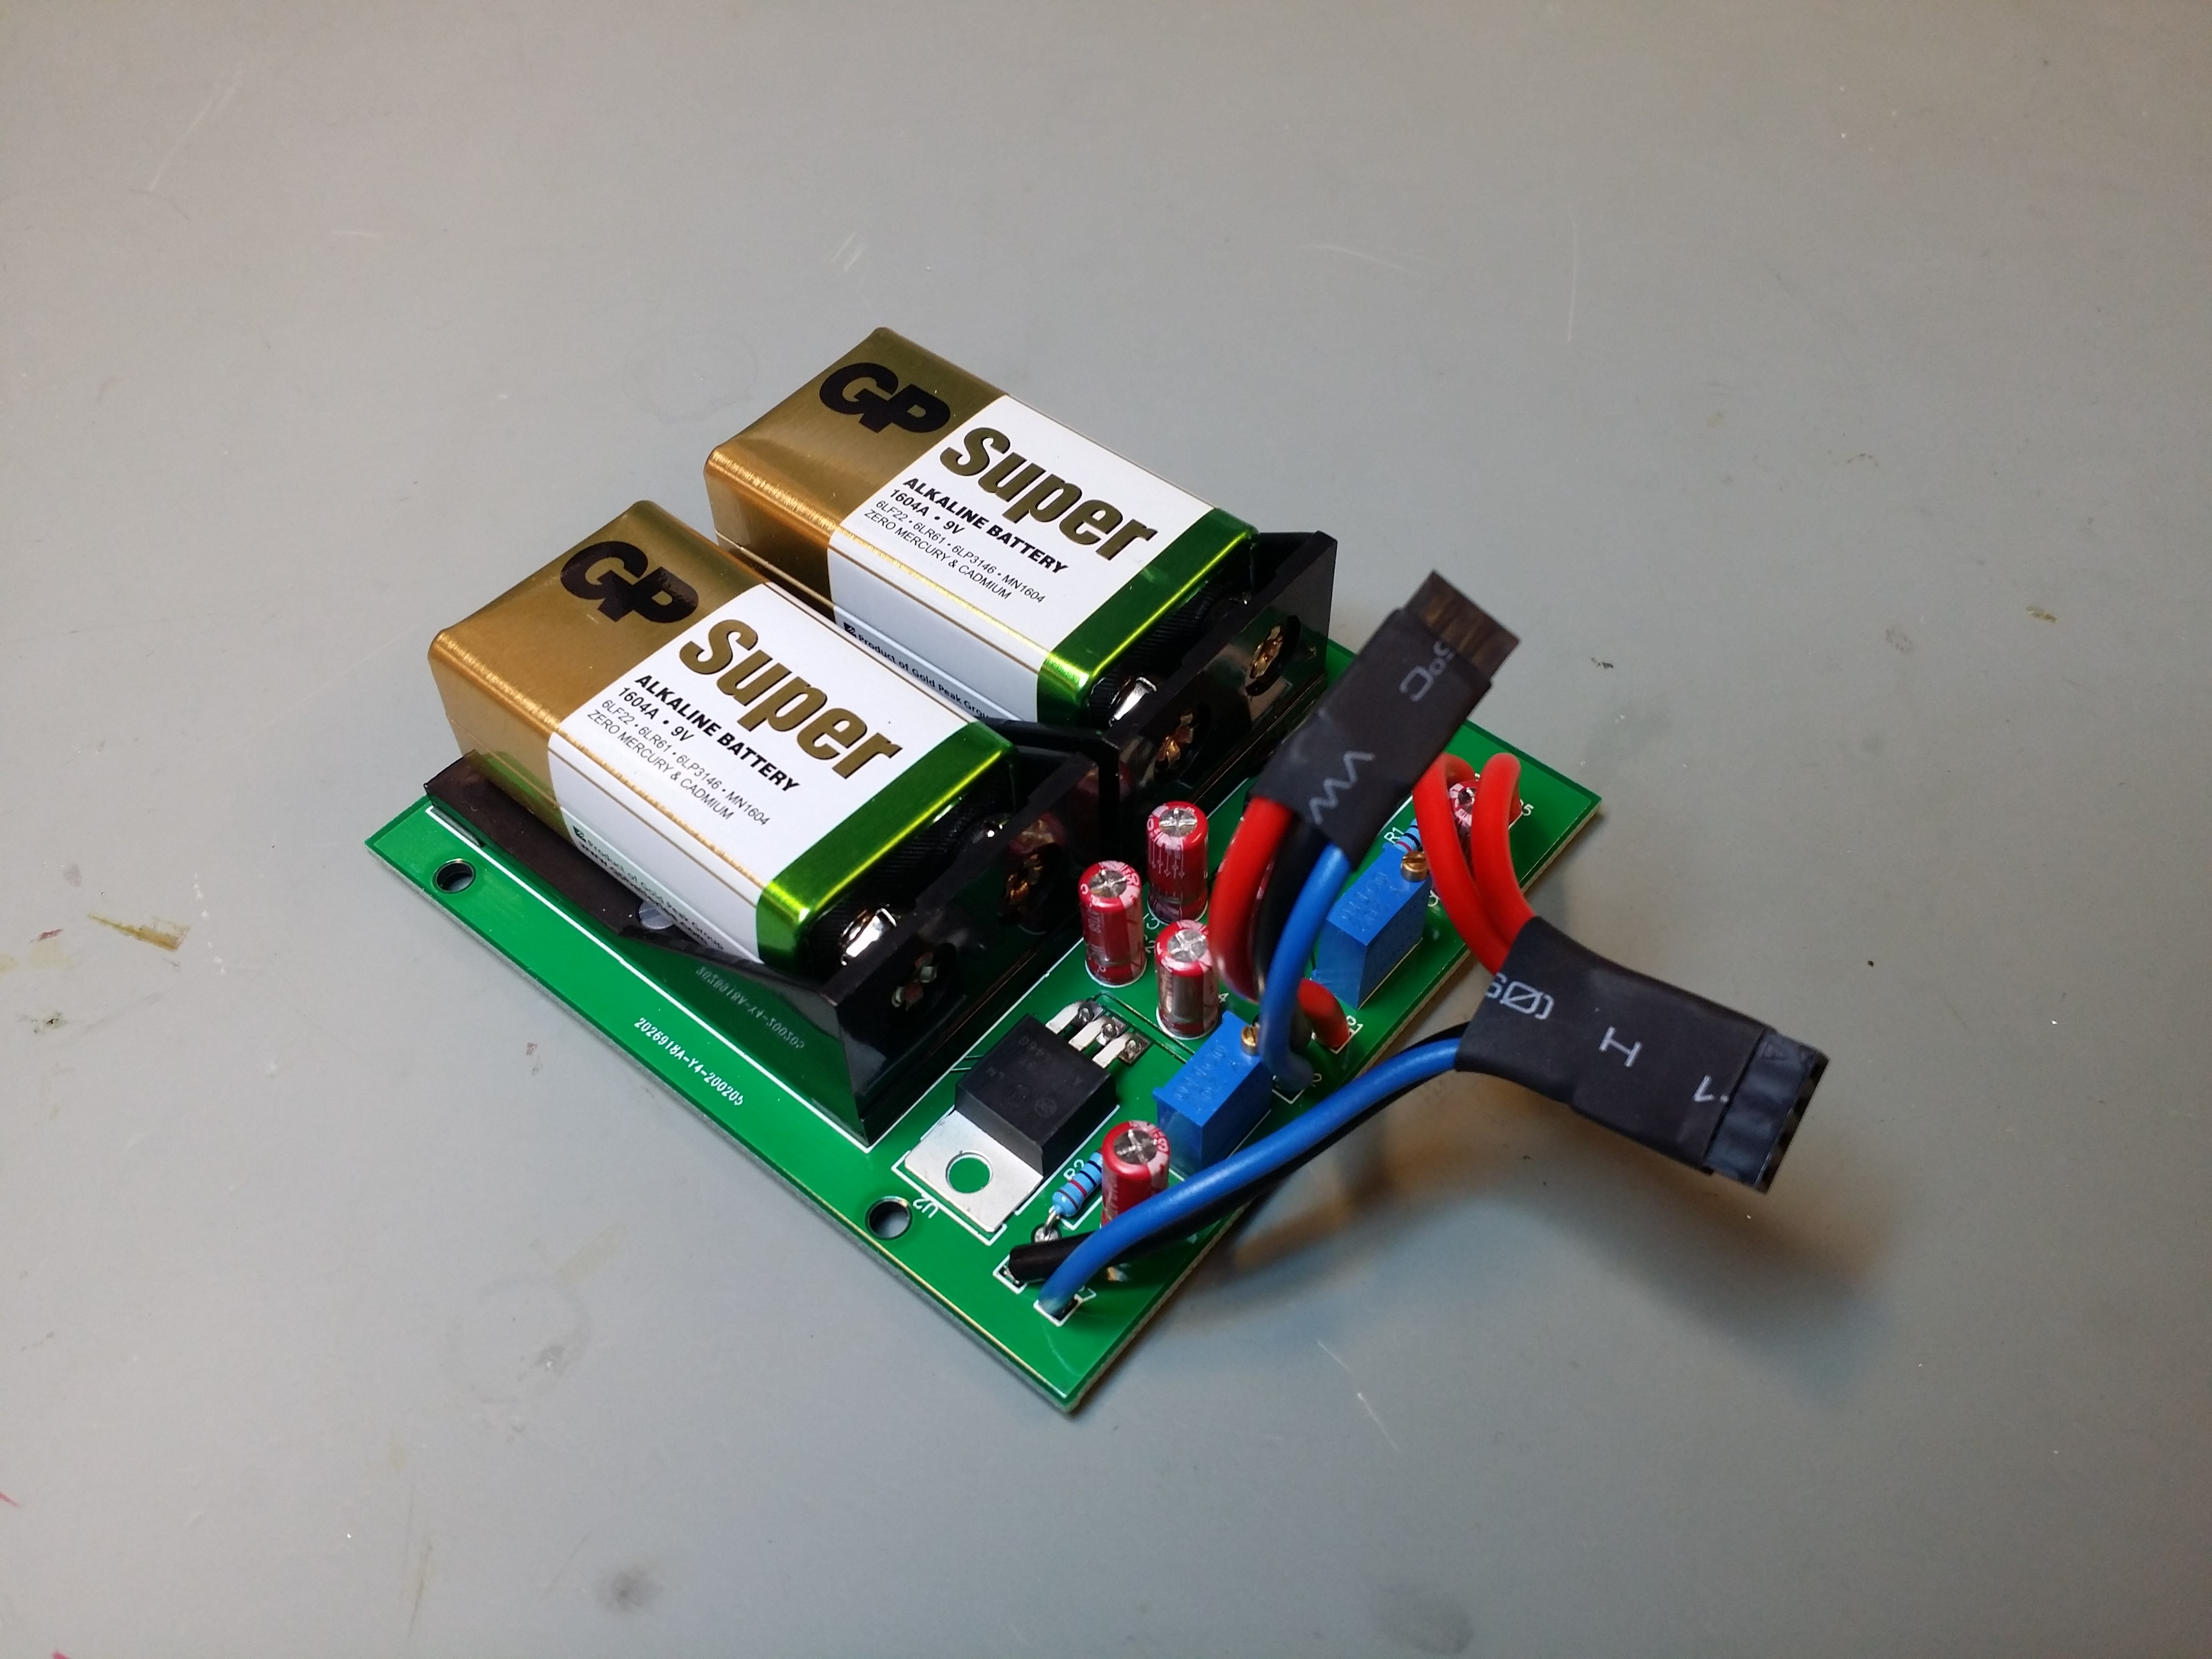
\includegraphics[width=\textwidth]{fig/IMG_20201201_121625.jpg}
}
\caption{Power supply for the pre-amplifier}
\end{figure}

\begin{figure}[ht!]
\centering
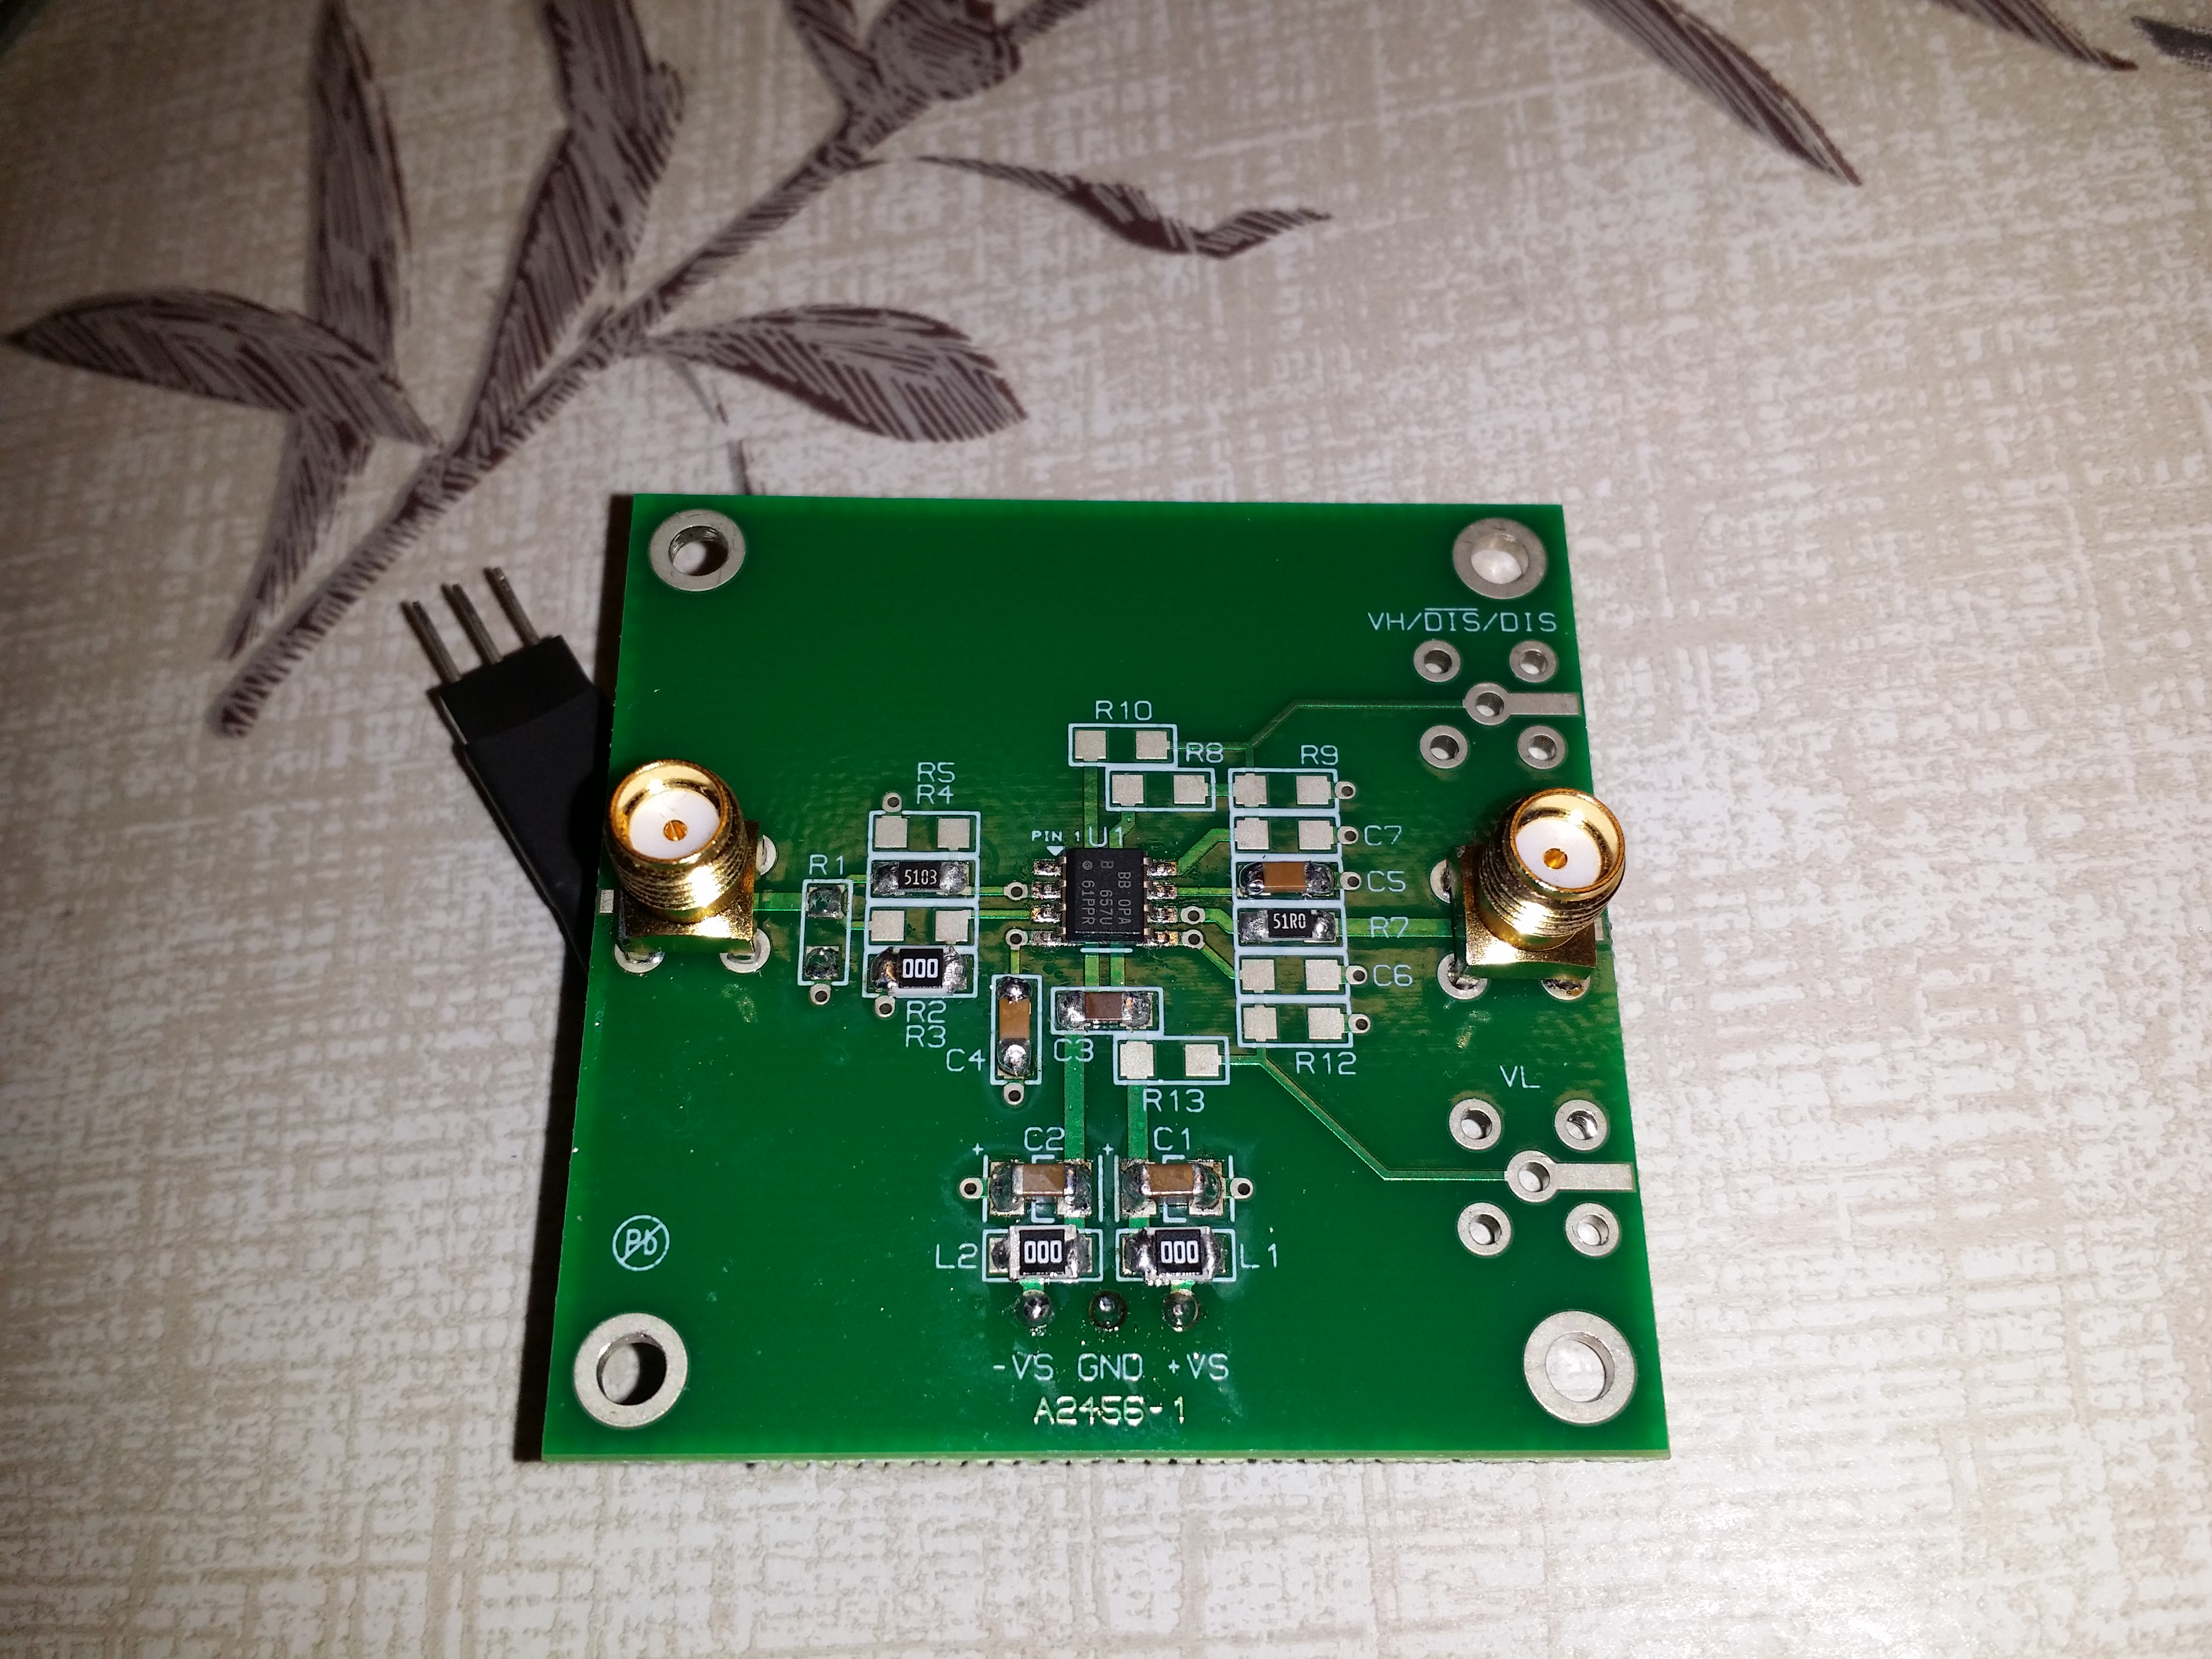
\includegraphics[width=\textwidth]{fig/IMG_20201207_121010.jpg}
\caption{Pre-amplifier board}
\end{figure}

\begin{figure}[ht!]
\centering
\subcaptionbox{}{
	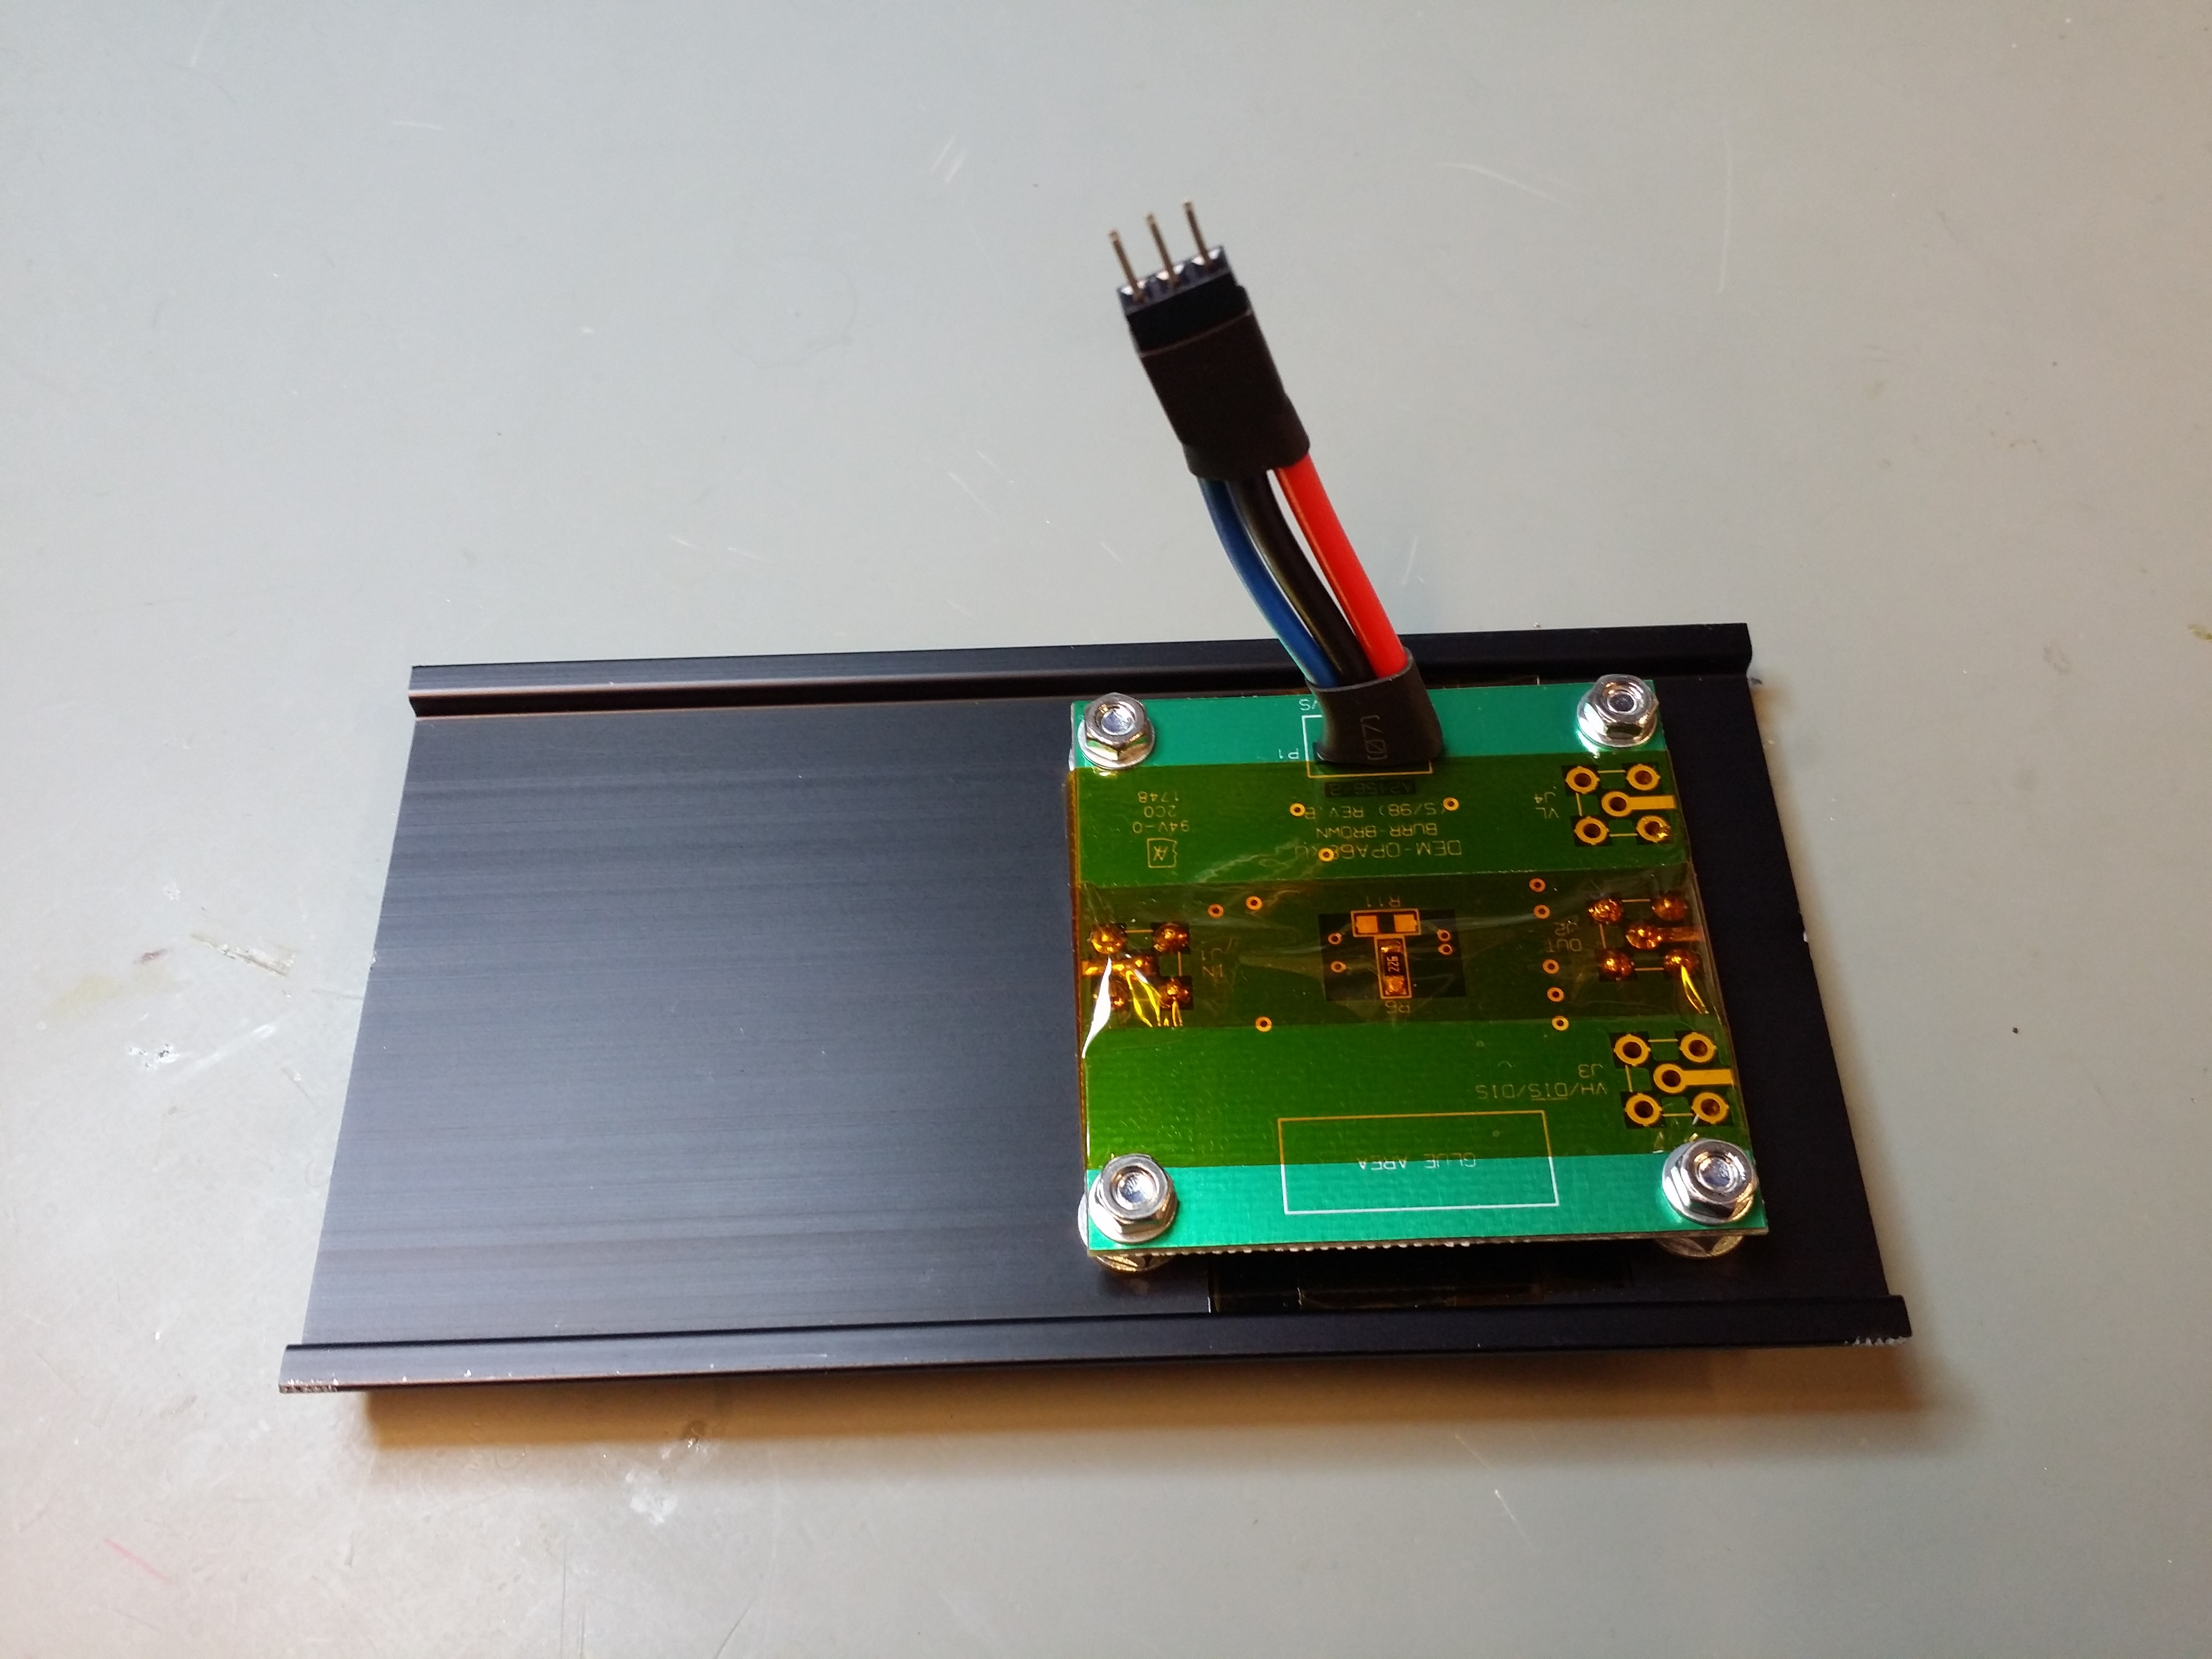
\includegraphics[width=\textwidth]{fig/IMG_20201201_121735.jpg}
}
\subcaptionbox{}{
	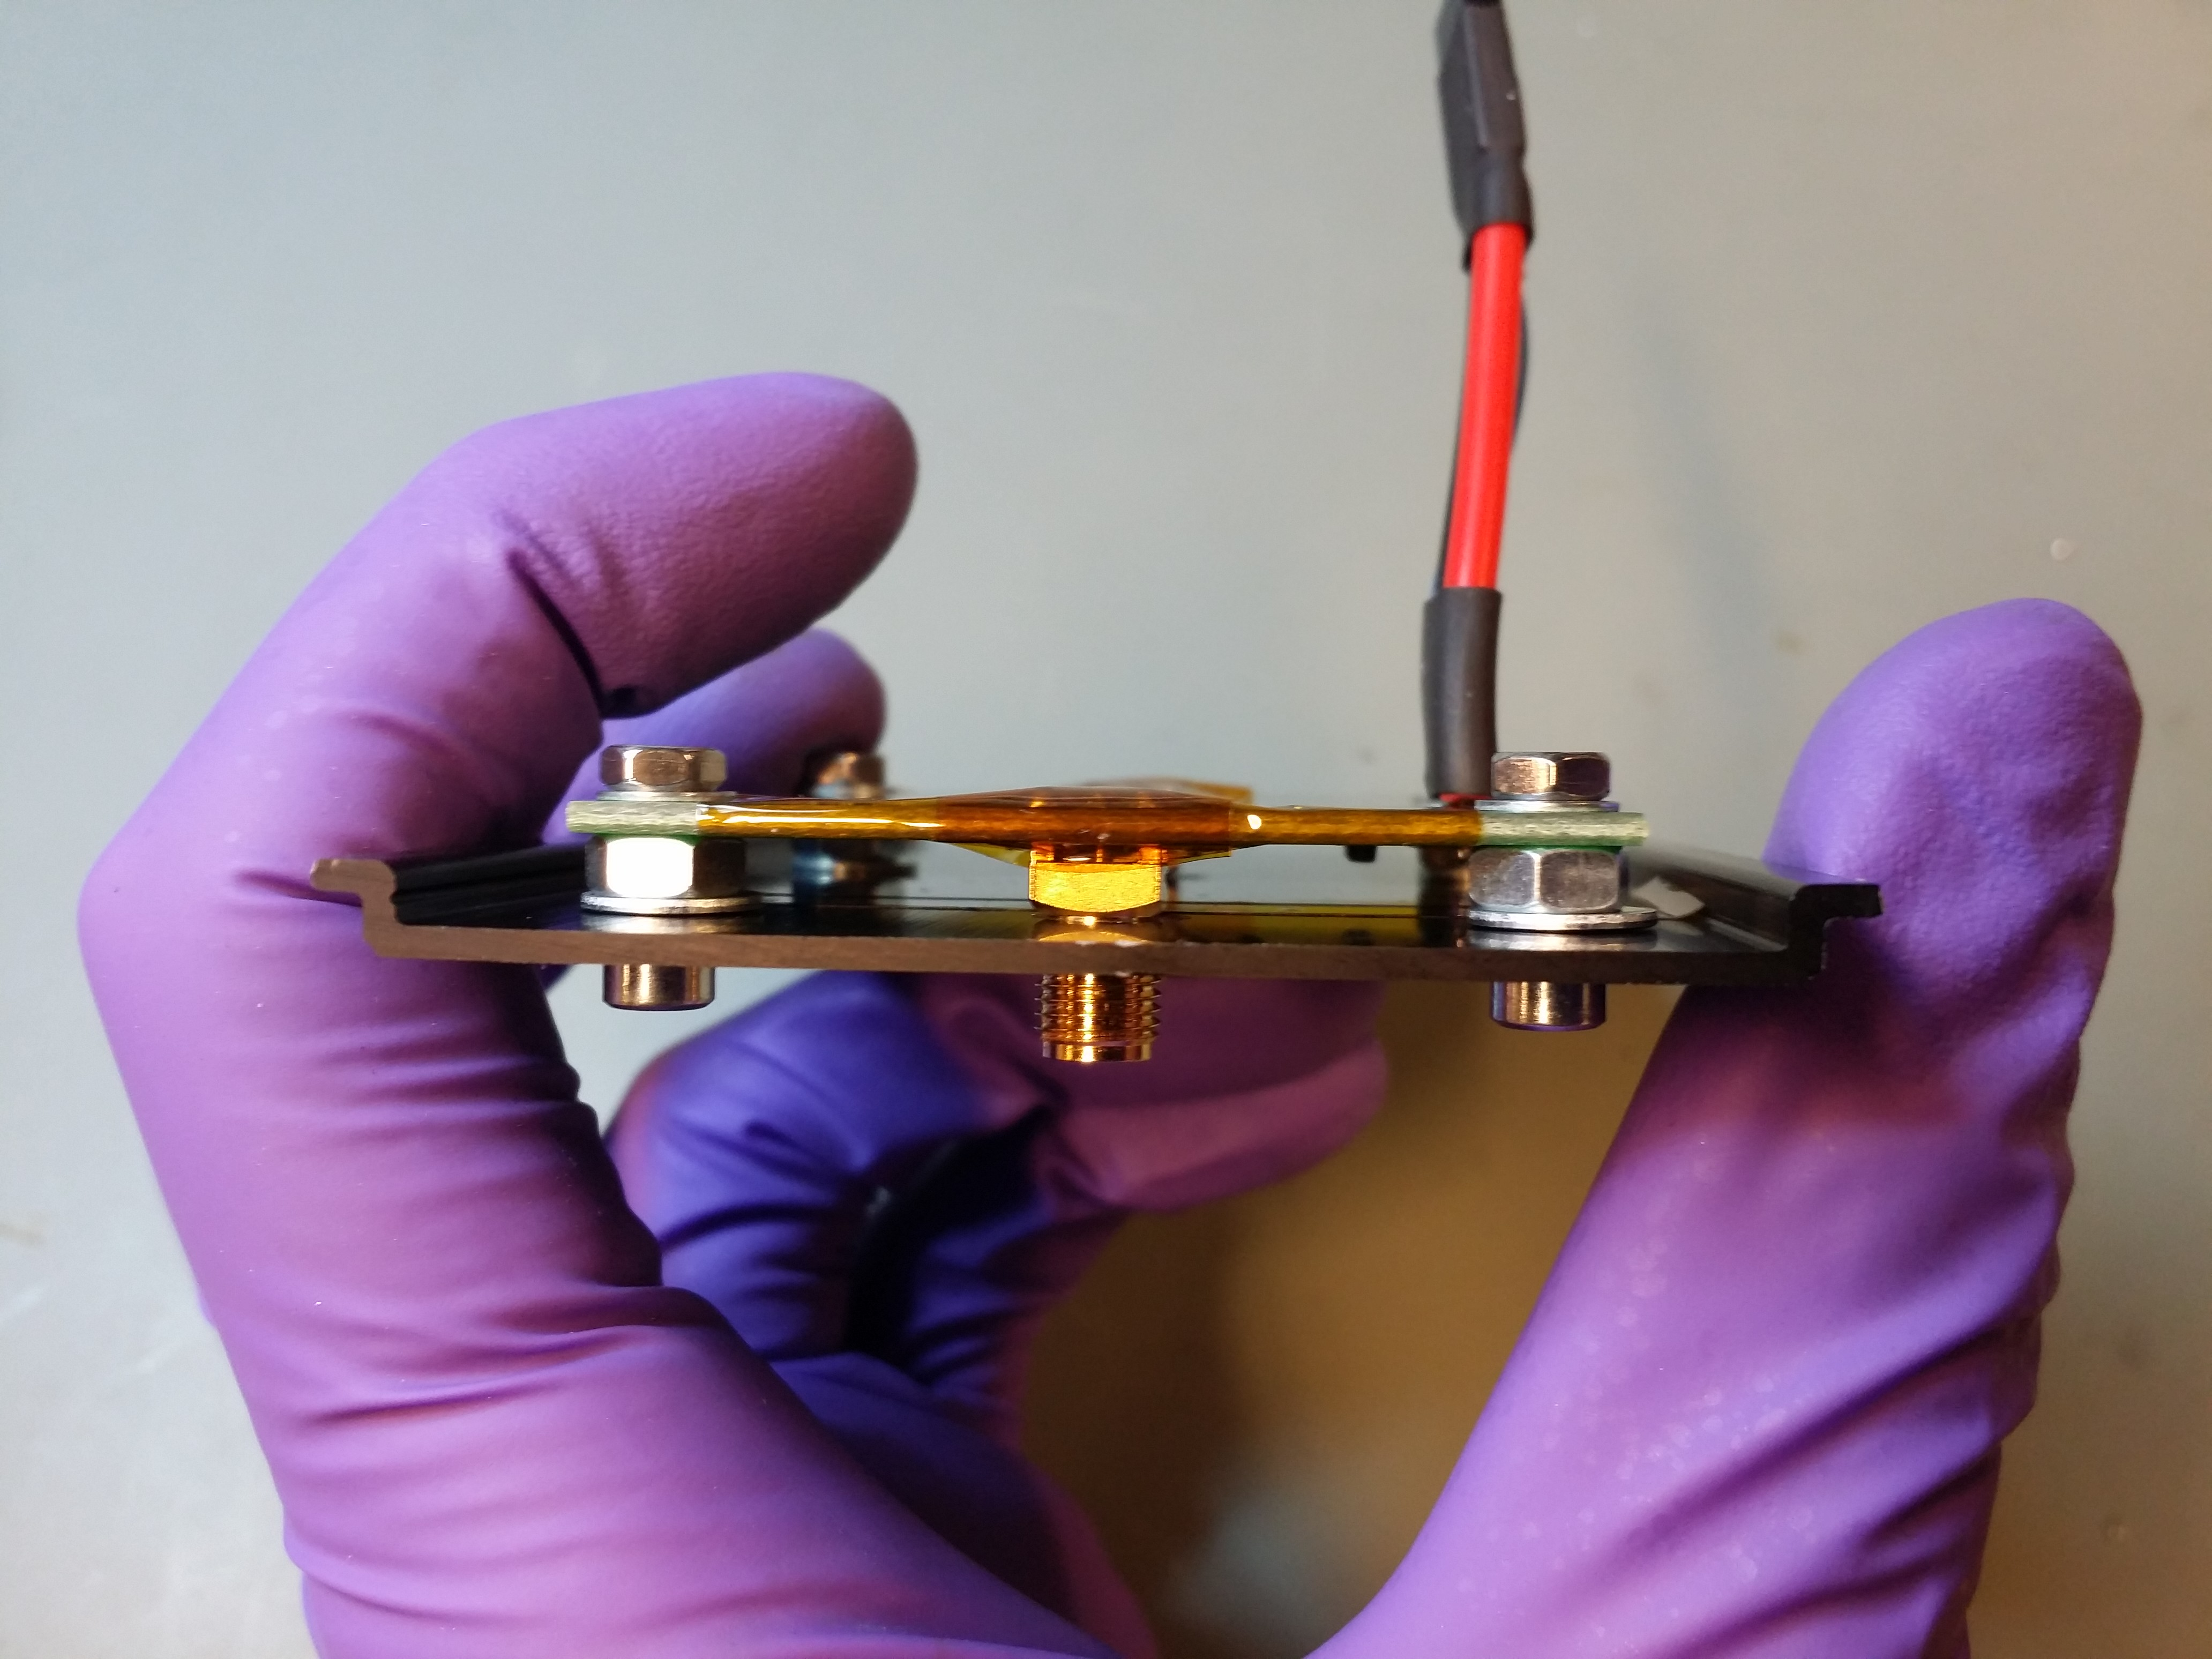
\includegraphics[width=\textwidth]{fig/IMG_20201201_121845.jpg}
}
\caption{Mounting of the pre-amplifier board}
\end{figure}

\end{appendices}


\clearpage
\section{References}
\printbibliography


\end{document}